%%%%%%%%%%%%%%%%%%%%%%%%%%%
% PREAMBOLO DEL DOCUMENTO %
%%%%%%%%%%%%%%%%%%%%%%%%%%%
\documentclass[a4paper,11pt,oneside,top=3cm,bottom=3cm,left=0cm,right=0cm,openright,reqno,table]{book}

% openany - fa iniziare i capitoli direttamente nella pagina successiva
% openright - fa iniziare i capitoli nella prima pagina destra disponibile 
% fleqn  - allinea le formule a sinistra anzichè centrarle
% leqno - dispone la numerazione delle formule sulla sinistra o destra
% reqno - dispone la numerazione delle formule sulla destra
%
\usepackage{packages}
% Per non appesantire troppo questo file
% quasi tutti i pacchetti usati sono salvati in packages.sty
%
\linespread{1.5}

% Per avere la parola BOZZA scritta su tutte le pagine

% funziona solo in modalità PS
% Invece per i PDF ho risolto così:
% pdftk tesi.pdf background bozza.pdf output tesi_bozza.pdf
%
%%%%%%%%%%%%%%%%%%%%%%%%%%%%%%%%%
%   DOCUMENTO VERO E PROPRIO    %
%%%%%%%%%%%%%%%%%%%%%%%%%%%%%%%%%
\begin{document}
% FRONTESPIZIO %
\begin{titlepage}
\changepage{}{}{}{}{}{}{}{}{}
% parametri per cambiare le dimensioni di una singola pagina in ordine:
% {textheight}{textwidth}{evensidemargin}{oddsidemargin}{columnsep}
% {topmargin}{headheight}{headsep}{footskip}
% se voglio centrare la pagina devo mettere bindingoffset/2
% i primi 5 parametri posso usarli con \changetext


\begin{center}

\includegraphics [width=.15\columnwidth, angle=0]{capitoli/images/unisa.pdf}\\ % height
\vspace{0.5cm}
{\LARGE \scshape Università degli Studi di Salerno}\\
\vspace{1cm}
{\Large Dipartimento di Informatica}\\
\vspace{2cm}
{\Large \scshape Statistica e Analisi dei Dati} \\
\vspace{2cm}
{\huge \bfseries Inferenza Statistica Distribuzione Normale} \\
\vspace{6cm}

\begin{minipage}[t]{7cm}
\flushleft
\textsc{Docente}

Prof.ssa \textbf{Amelia G. Nobile} \\[0.25cm]

\end{minipage}
\hfill
\begin{minipage}[t]{7cm}
\flushright
\textsc{Candidato}

\textbf{Mattia Mori} \\
Matricola: 0512105707
\end{minipage}

\vspace{2cm}

%& & \\
%& Candidato & \\
%& \textbf{Mattia Mori} & \\
{\small Anno Accademico 2022-2023} %\\

\end{center}

\end{titlepage}
\setlength{\headheight}{14pt}

\frontmatter
% quello che segue è in numerazione romana e i capitoli non verranno numerati
% se non si vuole che compaia il numero di pagina basta usare il comando:
%\nonumber

% RINGRAZIAMENTI %
\include{frontmatter/ringraziamenti}
% SOMMARIO %
\cleardoublepage
\include{frontmatter/sommario}
% INDICI %
\phantomsection
\addcontentsline{toc}{chapter}{Indice}
\tableofcontents
% Il simbolo * serve per evitare che comapaia nell'indice
\clearpage
%\listoffigures
%\clearpage
%\listoftables
% GLOSSARIO
%\cleardoublepage
\phantomsection
\addcontentsline{toc}{chapter}{Glossario}
% per inserire l'elenco dei simboli e degli acronimi nell'indice
\printglossary
% Per stampare il glossario
% per aggiornarlo si deve eseguire da terminale:
% makeindex -s myDoc.ist -t myDoc.alg -o myDoc.acr myDoc.acn
% per inserire una voce nell'elenco:
% \newglossaryentry{voce_etichetta}{name={voce}, description={descrizione}}
% se non compare direttamente nel testo va inizializzata con:
% \glsadd{voce_etichetta}
% oppure se viene richiamata all'interno del testo:
% \gls{voce_etichetta}
% SIMBOLI E NOTAZIONI %
%%%%%%%%%%%%%%%%%%%%%%%%%%%%%%%\cleardoublepage
\phantomsection
\addcontentsline{toc}{chapter}{Elenco delle tabelle}
% per inserire l'elenco dei simboli e degli acronimi nell'indice
%\printglossary[type=\acronymtype,title=Elenco delle figure]
% Per stampare l'elenco dei simboli
\listoftables
% per aggiornarlo si deve eseguire da terminale:
% makeindex -s myDoc.ist -t myDoc.glg -o myDoc.gls myDoc.glo
% per inserire una voce nell'elenco:
% \newglossaryentry{voce_etichetta}{name={voce}, description={descrizione}}
% se non compare direttamente nel testo va inizializzata con:
% \glsadd{voce_etichetta}
% oppure se viene richiamata all'interno del testo:
% \gls{voce_etichetta}

\mainmatter
% quello che segue sarà in numerazione araba e i capitoli verranno numerati
%\part{Studio iniziale}
% CAPITOLI
\phantomsection
\definecolor{dkgreen}{rgb}{0,0.6,0}
\definecolor{gray}{rgb}{0.5,0.5,0.5}
\definecolor{mauve}{rgb}{0.58,0,0.82}


\lstset{frame=tb,
language=R,
aboveskip=3mm,
belowskip=3mm,
showstringspaces=false,
columns=flexible,
numbers=none,
inputencoding=utf8/latin1,
keywordstyle=\color{blue},
numberstyle=\tiny\color{gray},
commentstyle=\color{dkgreen},
stringstyle=\color{mauve},
breaklines=true,
breakatwhitespace=true,
tabsize=3
}

\chapter{Introduzione}

Si possono ottenere le caratteristiche di una popolazione limitata mediante l'osservazione della totalità delle entità della popolazione o di un suo sottoinsieme, denominato "campione". Nel caso di una popolazione illimitata, è possibile lo studio solo mediante un campione di questa. Lo scopo dell'inferenza statistica è quello di estendere le misure ottenute dall'analisi di un campione a tutta la popolazione di cui il campione fa parte, accertandosi che il campione sia idoneo e rappresentativo per la popolazione.

L'\textit{inferenza statistica} si basa su due metodi fondamentali di indagine:

\begin{itemize}
    \item \textit{stima dei parametri}
    \item \textit{verifica delle ipotesi}
\end{itemize}

La \textit{stima dei parametri} ha lo scopo di determinare i valori non noti dei parametri di una popolazione, cioè il valore medio e la varianza, impiegando i parametri corrispondenti ottenuti dal campione. Questi parametri possono essere stimati utilizzando le \textit{stime puntuali} o le \textit{stime per intervallo}.

Per quanto riguarda la verifica delle ipotesi, consiste nella realizzazione di un'ipotesi sul parametro non noto e decidere la sua accettabilità in base ai risultati ottenuti dal campione estratto.

Per sfruttare l'inferenza statistica, l'analisi verterà sullo studio di un campione di una popolazione avente distribuzione normale. Si noti che R mette a disposizione per ogni distribuzione le seguenti funzioni:

\begin{itemize}
    \item $d$ calcola la funzione di probabilità di una variabile aleatoria in uno specifico punto o in un insieme di punti (density mass);
    \item $p$ calcola la funzione di distribuzione di una variabile aleatoria in uno specifico punto o in un insieme di punti (probability distribution);
    \item $q$ calcola la funzione quantili;
    \item $r$ simula una variabile aleatoria mediante la generazione di numeri pseudocasuali.
\end{itemize}

\section{Variabile Aleatoria Normale}

Nelle variabili aleatorie casuali continue è importante conoscere la probabilità che uno specifico valore sia compreso in un determinato intervallo.

\noindent \textbf{Definizione:} Una variabile aleatoria X di densità di probabilità

\[f_X(x) = \frac{1}{\sigma \sqrt{2\pi}}e^{-\frac{(x-\mu)^2}{2\sigma^2}}, \quad x \in \mathbb{R}, \quad (\mu \in \mathbb{R}, \sigma \> 0) \]

si dice avente distribuzione normale o di Gauss, di parametri $\mu$ (valore medio) e $\sigma$ (deviazione standard), principalmente utilizzata per la descrizione di fenomeni fisici e biologici.

La notazione del tipo $X ~ N(\mu, \sigma)$ indica che la $X$ ha distribuzione normale dei parametri $\mu$ e $\sigma$, o più semplicemente che è una variabile normale. Ci sono alcune proprietà che vengono soddisfatte dalla densità di probabilità normale, che sono:

\begin{itemize}
    \item simmmetria rispetto all'asse $x = \mu \forall x \in \mathbb{R} fx(\mu - x) = fx(\mu + x)$
    \item massimo nel punto di ascissa $x = \mu$ e nello specifico in $(\sigma \sqrt{2\pi})^{-1}$
    \item due punti di flesso nei punti $(\mu - \sigma)(\mu + \sigma)$
\end{itemize}

In R il calcolo della densità di probabilità di una variabile 
$X ~ N(\mu, \sigma)$ si può calcolare tramite la funzione \textit{dnorm}, la quale accetta come valori:

\begin{itemize}
    \item x, valori assunti dalla variabile aleatoria normale;
    \item mean e sd sono rispettivamente il valore medio e la deviazione standard della densità normale;
\end{itemize}

Il codice di seguito mostra come ottenere la densità di probabilità di una variabile aleatoria normale:

\vspace{5mm}
\begin{lstlisting}
  curve(dnorm(x, mean = -3, sd = 1),
        from = -6, to = 6, xlab = "x", ylab = "f(x)",
        main = " mu = [-3, -2, -1, 0, 1, 2, 3]; sigma = 1")
  curve(dnorm(x, mean = -2, sd = 1),
        from = -6, to = 6, xlab = "x",
        ylab = "f(x)", add = TRUE)
  curve(dnorm(x, mean = -1, sd = 1),
        from = -6, to = 6, xlab = "x",
        ylab = "f(x)", add = TRUE)
  curve(dnorm(x, mean = 0, sd = 1),
        from = -6, to = 6, xlab = "x",
        ylab = "f(x)", add = TRUE, lty = 2)
  curve(dnorm(x, mean = 1, sd = 1),
        from = -6, to = 6, xlab = "x",
        ylab = "f(x)", add = TRUE)
  curve(dnorm(x, mean = 2, sd = 1),
        from = -6, to = 6, xlab = "x",
        ylab = "f(x)", add = TRUE)
  curve(dnorm(x, mean = 3, sd = 1),
        from = -6, to = 6, xlab = "x",
        ylab = "f(x)", add = TRUE)
\end{lstlisting}
\vspace{5mm}

\begin{figure}[!htb]
    \centering
    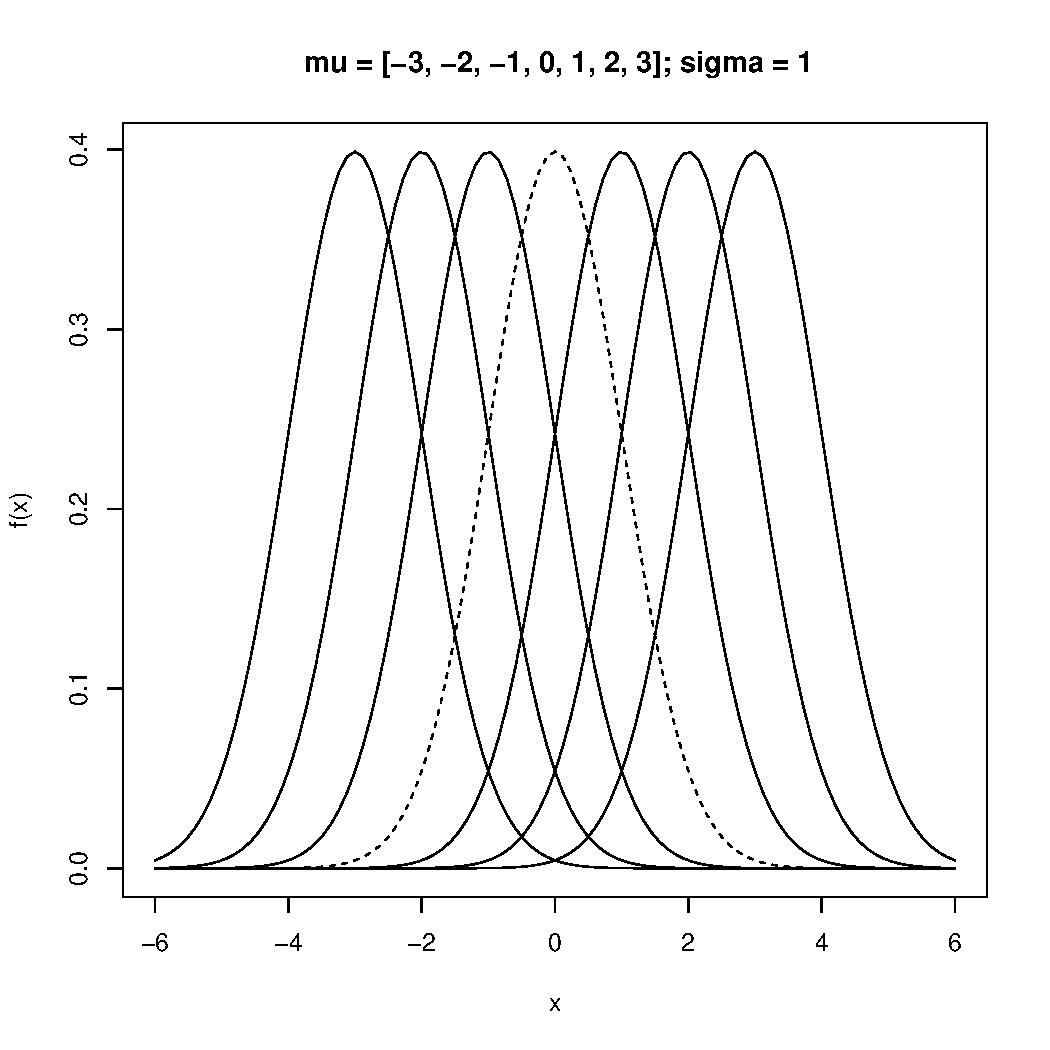
\includegraphics[height=16cm]{capitoli/images/1_introduzione/dens_prob_val.pdf}
    \caption{Densità normale.}
\end{figure}

Le variazioni al parametro $\mu$ comportano la traslazione della curva lungo tutto l'asse delle ascisse, senza cambiare la propria forma, mentre il parametro $\sigma$ caratterizza la larghezza della funzione. Poiché la massima ordinata è inversamente proporzionale a $\sigma$, decresce al crescere di $\sigma$ stesso mentre l'area sottesa della curva deve rimanere unitaria.

Quando $\mu = 0$ e $\sigma = 1$ possiamo ottenere la \textit{variabile aleatoria normale standardizzata.}

\vspace{5mm}
\begin{lstlisting}
  curve( dnorm(x,mean=0,sd=1), from=-6, to=6, xlab="x", ylab="f(x)", main="mu= 0, sigma=1")
\end{lstlisting}
\vspace{5mm}

\begin{figure}[!htb]
    \centering
    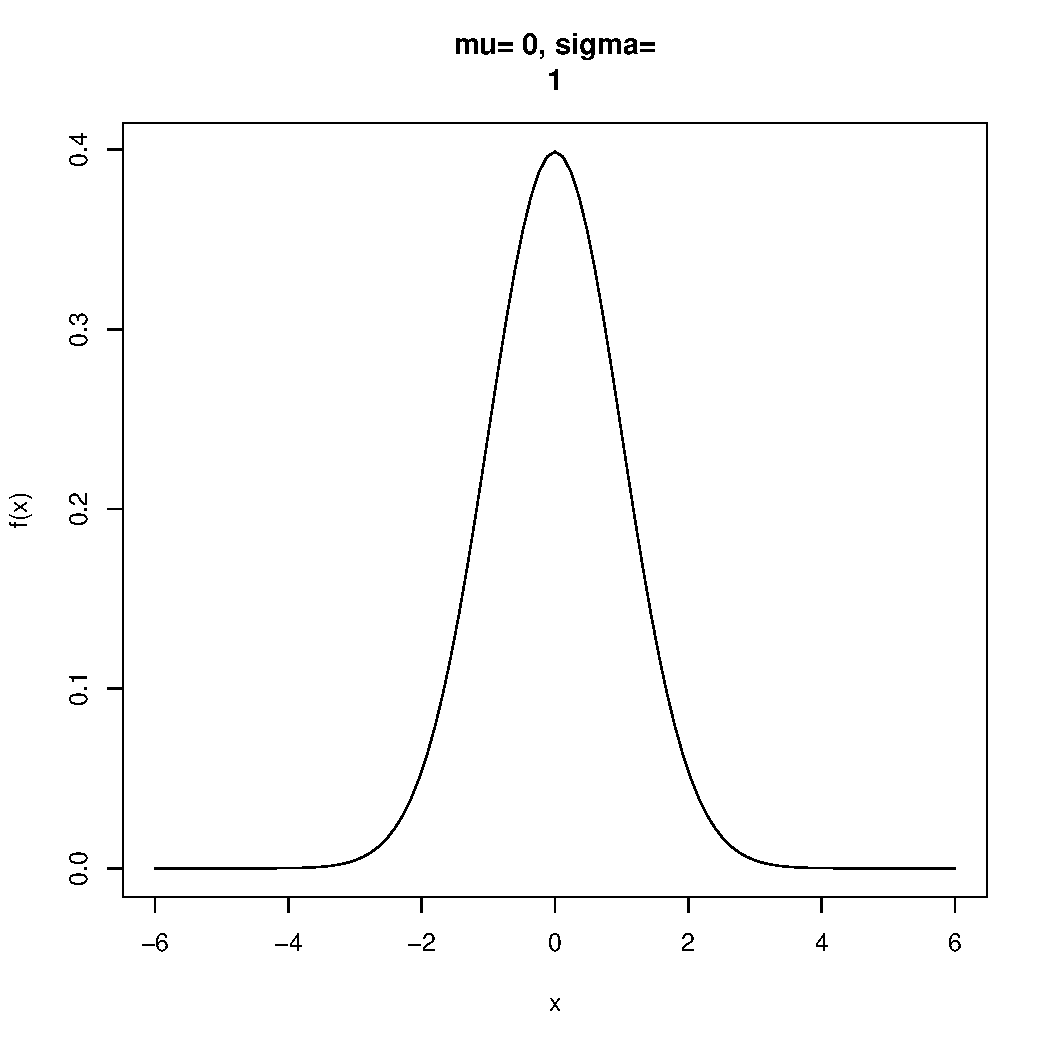
\includegraphics[height=16cm]{capitoli/images/1_introduzione/var_norm_stand.pdf}
    \caption{Variabile normale standard.}
\end{figure}

La funzione di distribuzione standard di uan variabile aleatoria $X ~ N(\mu, \sigma)$ è:

\[F_x(x) = P(X \leq x) = \int_{-\inf}^{x}fx(y)dy = \phi(\frac{x - \mu}{\sigma}) \quad x \in \mathbb{R}\]

dove 

\[\phi(z) = \frac{1}{\sqrt{2\pi}} \int_{-\inf}^z exp\{-\frac{y^2}{2}\}dy \quad z \in \mathbb{R}\]

è la funzione di distribuzione di una variabile aleatoria $Z ~N (0, 1)$

In R la funzione di distribuzione di una variabile $X \sim N(\mu, \sigma)$ può essere calcolata mediante l'impiego della funzione \textit{pnorm} la quale accetta come valori:

\begin{itemize}
    \item x, valori assunti dalla variabile aleatoria normale;
    \item mean e sd sono rispettivamente il valore medio e la deviazione standard della densità normale;
    \item lower.tail se TRUE calcola $P(X\leq x)$, se FALSE calcola $P(X \> x)$;
\end{itemize}

Il seguente codice mostra la funzione di distribuzione di una variabile aleatoria normale standard:

\vspace{5mm}
\begin{lstlisting}
  curve(pnorm(x, mean = 0, sd = 1), from = -4, to = 4, xlab = "x",
        ylab = expression(P(X <= x)), main = " mu = 0; sigma = 1", lty = 2)
  curve(pnorm(x, mean = 0, sd = 1), add = TRUE)
\end{lstlisting}
\vspace{5mm}

\begin{figure}[!htb]
    \centering
    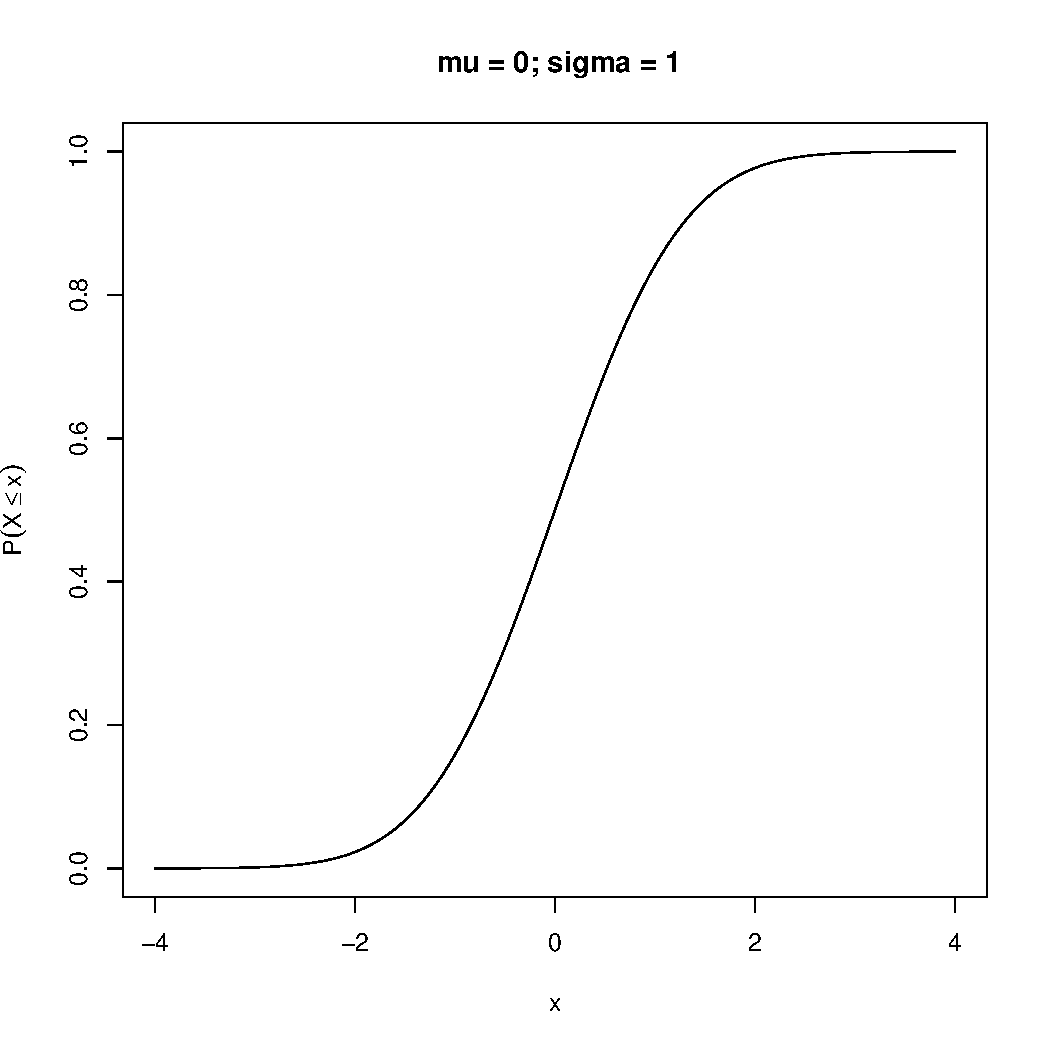
\includegraphics[height=16cm]{capitoli/images/1_introduzione/dist_var_norm_stand.pdf}
    \caption{Funzione di distribuzione della normale standard.}
\end{figure}


\section{Generazione del dataset}

Per generare il dataset si è utilizzata la funzione \textit{rnorm}.

\vspace{5mm}
\begin{lstlisting}
ds <- rnorm(80, 2, 0.5)

 [1] 2.5889415 2.4274552 2.2879886 2.5257274 1.3608815 1.8330865 2.2110392
 [8] 2.9302882 2.1603784 2.8153400 1.2379034 1.3232095 1.5533711 1.1738130
[15] 1.1798547 2.0803117 1.4592185 1.5569350 1.4902865 2.0316545 2.4187870
[22] 2.5316882 3.0833015 1.8875859 1.5517724 3.0869650 2.1161441 2.2039643
[29] 1.0669755 2.0200946 2.5388058 2.3822110 2.1206882 1.6142661 2.3803540
[36] 2.4263595 2.8091048 1.5316683 1.6807372 2.7404029 1.5801006 1.8411243
[43] 1.9379254 2.2090764 1.8581314 2.2168108 2.4149075 1.8682822 2.4080365
[50] 2.5663934 1.7010245 1.8328371 1.9498204 1.5384879 1.6274098 2.4448616
[57] 1.6637135 3.1919928 1.2788193 1.6247899 1.8259281 2.1353790 2.0575756
[64] 2.2415920 2.6733718 1.0493558 1.7638138 2.3932882 1.8392844 2.2664697
[71] 1.8736283 1.3277308 1.8608656 2.1320640 1.3944918 1.5087226 2.2219716
[78] 0.9680605 2.1960015 1.8015670
\end{lstlisting}
\vspace{5mm}

In questo caso è stato generato un campione formato da 80 elementi con $\mu = 2$ e $\sigma = 0.5$.
Ovviamente si suppone che il seguente campione sia stato estratto dalla popolazione e che esso sia rappresentativo di quest'ultima. Del dataset appena creato se ne calcola il valore medio $\mu$ e la deviazione standard $\sigma$.

\vspace{5mm}
\begin{lstlisting}
mu <- round(mean(ds), digits = 2)
mu
[1] 2

sigma <- round(sd(ds), digits = 2)
sigma
[1] 0.51
\end{lstlisting}
\vspace{5mm}

Una volta calcolati tali valori è possibile disegnare la variabile aleatoria normale che approssima il nostro campione attraverso la funzione dnorm:

\vspace{5mm}
\begin{lstlisting}
  curve(dnorm(x, mean = mu, sd = sigma), from = 0, to = 10, xlab = " x", ylab = "f(x)",
        main = paste("mu: ", mu, " sigma: ", sigma))
  lines(x = c(mu - sigma, mu, mu + sigma), y = dnorm(c(mu - sigma, mu, mu + sigma), mu, sigma),
        type = "h", lty = 2, col = c("green", "red", "green"), xlab = "")
  axis(1, at = c(mu - sigma, mu, mu + sigma), c("(mu - sigma)", "mu", "(mu + sigma)"))
\end{lstlisting}
\vspace{5mm}

\begin{figure}[!htb]
    \centering
    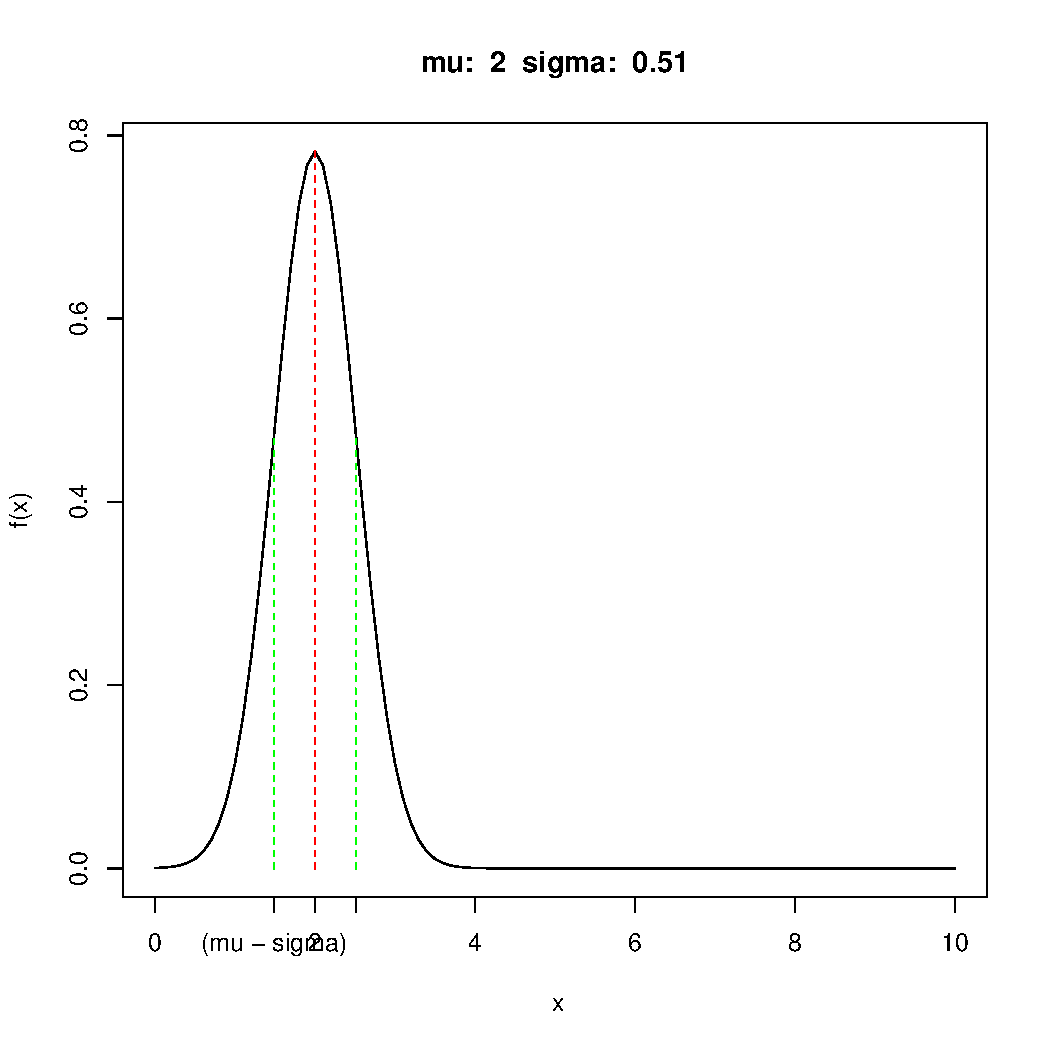
\includegraphics[height=16cm]{capitoli/images/1_introduzione/appross_dataset_norm.pdf}
    \caption{Approssimazione del dataset con la normale.}
    \label{app_data_norm}
\end{figure}

ottenendo la \ref{app_data_norm}, nella quale sono stati evidenziati in rosso il valore medio $\mu$ e in verde i due punti di flesso $(\mu - \sigma)$ e $(\mu + \sigma)$.






%################################################

\newpage
\phantomsection
\definecolor{dkgreen}{rgb}{0,0.6,0}
\definecolor{gray}{rgb}{0.5,0.5,0.5}
\definecolor{mauve}{rgb}{0.58,0,0.82}


\lstset{frame=tb,
language=R,
aboveskip=3mm,
belowskip=3mm,
showstringspaces=false,
columns=flexible,
numbers=none,
inputencoding=utf8/latin1,
keywordstyle=\color{blue},
numberstyle=\tiny\color{gray},
commentstyle=\color{dkgreen},
stringstyle=\color{mauve},
breaklines=true,
breakatwhitespace=true,
tabsize=3
}

\chapter{Stima dei parametri Distribuzione Normale}

\section{Stima puntuale}

Una problematica particolare che riguarda l'inferenza statistica riguarda il voler studiare una popolazione descritta da una variabile aleatoria osservabile $X$ con una funzione di distribuzione nota ma con un parametro $\theta \in \Theta$ non noto (o più parametri)

\subsection{Metodi per la ricerca di stimatori}

Nei metodi di indagine per l'inferenza statistica, a partire da un campione casuale $X_1, X_2, ..., X_n$ di ampiezza $n$ estratto dalla popolazione si cerca di ottenere informazioni sul parametro non noto $\theta$ mediante l'uso di alcune variabili aleatorie, chiamate \textit{stimatori}, che sono funzioni misurabili del campione casuale.

\noindent \textbf{Definizione:} Uno stimatore $\hat{\theta} = t(X_1, X_2, ..., X_n)$ è una funzione misurabile e osservabile del campione casuale $X_1, X_2, ..., X_n$ i cui valori possono essere usati per stimare un parametro non noto $\theta$ della popolazione. I valori $\hat{\theta}$ assunti da tale stimatore sono detti \textit{stime} del parametro non noto $\theta$. Alcune statistiche tipiche sono la media campionaria e la varianza campionaria.

\subsection{Metodo dei momenti}

Per stimare i parametri non noti, viene impiegato il Metodo dei momenti.

\textbf{Definizione:} Si definisce momento campionario r-esimo relativo ai valori osservati ($x_1, x_2, ..., x_n$) del campione casuale il valore

\[M_r(x_1, x_2, ..., x_n) = \frac{1}{n}\sum_{i=1}^n x_i^r \quad (r = 1, 2, ..., k)\]

Dalla definizione il momento campionario r-esimo è la media aritmetica delle potenze r-esime delle n osservazioni effettuate sulla popolazione. Dunque, con $r = 1$, il momento campionario coincide con il calore osservato dalla media campionaria $\Bar{X}$.

Con k parametri da stimare, uguagliamo i primi k momenti della popolazione con i corrispondenti momenti del campione casuale: se i primi k momenti esistono e sono finiti, il metodo dei momenti si riduce alla risoluzione di un sistema di k equazioni:

\[E(X^r) = M_r(x_1, x_2, ..., x_n) \quad (r = 1, 2, ..., k)\]

Le incognite del sistema sono i parametri $\theta, \theta, ..., \theta$ ed essendo una stima di tali incognite vengono indicati con $\hat{\theta}$. Gli stimatori $\hat{\Theta}$ dei parametri non noti, definiti \textit{stimatori del metodo dei momenti}, sono ottenuti al variare dei possibili campioni osservati.

\vspace{5mm}
\noindent \textbf{Popolazione normale}

Con il metodo dei momenti, si è interessati dunque a determinare gli stimatori dei parametri $\mu$ e $\delta^2$ di una popolazione normale di densità di probabilità

\[f_X(x) = \frac{1}{\delta \sqrt{2\pi}} e^{-\frac{(x - \mu)^2}{{2\delta}^2}}, \quad x \in \mathbb{R}, (\mu \in \mathbb{R}, \delta > 0)\]

L'applicazione del metodo dei momenti per la risoluzione del sistema $M_r$ permette di ottenere come stimatore del valore medio $\mu$ la media campionaria $\Bar{X}$ e come stimatore della varianza $\delta^2$ la variabile aleatoria $(n-1)S^2/n$.

\vspace{5mm}
\noindent \textbf{Metodo dei momenti - applicazione dataset}

Applicando il metodo dei momenti al campione in esame descritto da una variabile aleatoria normale, si ottiene: 

\vspace{5mm}
\begin{lstlisting}
  stima_mu <- mean(ds)
  stima_mu
  [1] 1.996316

  stima_s2 <- round((length(ds) - 1) * var(ds) / length(ds), digits = 2)
  stima_s <- sqrt(stima_s2)
  stima_s
  [1] 0.509902
\end{lstlisting}
\vspace{5mm}

La stima del parametro $\mu$ con il metodo dei momenti è $\hat{\mu} = 1.996316$ e la stima del parametro $\delta$ con il metodo dei momenti è $\hat{\delta} = 0.509902$. Come è possibile notare dal codice è stata presa in considerazione la deviazione standard $\delta$ effettuando quindi la radice della varianza.

\subsection{Metodo della massima verosimiglianza}

Il metodo della massima verosimiglianza è il più importante per la stima dei parametri non noti di una popolazione e viene solitamente preferito al metodo dei momenti. Al fine di illustrare questo metodo, occorre introdurre la funzione di verosimiglianza

\noindent \textbf{Definizione:} Sia $X_1, X_2, ..., X_n$ un campione casuale di ampiezza n estratto dalla popolazione. La funzione di verosimiglianza $L(\theta_1, \theta_2, ..., \theta_k) =L(\theta_1, \theta_2, ..., \theta_k ; x_1, x_2, ..., x_n)$ del campione osservato $(x_1, x_2, ..., x_n)$ è la funzione di probabilità congiunta (nel caso di popolazione discreta) oppure la funzione densità di probabilità congiunta (nel caso di popolazione assolutamente continua) del campione casuale $X_1, X_2, ..., X_n$, ossia:

\[L(\theta_1, \theta_2, ..., \theta_k) =L(\theta_1, \theta_2, ..., \theta_k ; x_1, x_2, ..., x_n) \]
\[= f(x_1;\theta_1, \theta_2, ..., \theta_k) f(x_2;\theta_1, \theta_2, ..., \theta_k) ... f(x_n;\theta_1, \theta_2, ..., \theta_k)\]

Il metodo della massima verosimiglianza consiste nella massimizzazione della funzione di verosimiglianza rispetto ai parametri $\theta_1, \theta_2, ..., \theta_k$, cercando di determinare da quale funzione di probabilità congiunta (nel caso di una popolazione discreta) oppure di densità di probabilità congiunta (nel caso di popolazione assolutamente continua) è più verosimile (plausibile) che provenga il campione osservato ($x_1, x_2, ...., x_n$). Pertanto, si cercano di determinare i valori $\theta_1, \theta_2, ..., \theta_k$ che rendono massima la funzione di verosimiglianza, offrendo in un certo senso la migliore spiegazione del campione osservato ($x_1, x_2, ..., x_n$).

I valori di $\theta_1, \theta_2, ..., \theta_k$ che massimizzano la funzione di verosimiglianza sono indicati con $\hat\theta_1, \hat\theta_2, ..., \hat\theta_k$ e costituiscono le stime di massima verosimiglianza dei parametri non noti $\theta_1, \theta_2, ..., \theta_k$ della popolazione. Tali stime dipendono dal campione osservato $(x_1, x_2, ..., x_n)$ e quindi al variare dei possibili campioni osservati si ottengono gli stimatori della massima verosimiglianza $\hat\theta_1, \hat\theta_2, ..., \hat\theta_k$ dei parametri non noti $\theta_1, \theta_2, ..., \theta_k$ della popolazione, detti \textit{stimatori di massima verosimiglianza}.

\vspace{5mm}
\noindent \textbf{Popolazione normale}

Si desidera determinare lo stimatore di massima verosimiglianza dei parametri $\mu$ e $\delta^2$ di una popolazione normale caratterizzata da funzione densità di probabilità

\[f_x(x) = \frac{1}{\sqrt{2\pi \delta^2}} exp\{-\frac{(x - \mu)^2}{2\delta^2}\} \quad (x \in \mathbb{R}, \mu \in \mathbb{R}, \delta > 0)\]

si ha

\[L(\mu, \delta^2) = (\frac{1}{\sqrt{2\pi \delta^2}}^n exp\{-\sum_{i=1}^n \frac{(x_i - \mu)^2}{2\delta^2}\} \quad (\mu \in \mathbb{R}, \delta > 0)\]

dove le $x_i \in \mathbb{R}$. Si nota che

\[log L(\mu, \delta^2) = -\frac{n}{2}log\delta^2 - \frac{n}{2}log(2\pi) - \frac{1}{2\delta^2}\sum_{i=1}^n(x_i - \mu)^2 \quad (\mu \in \mathbb{R}, \delta > 0)\]

e quindi si ha

\[\frac{\theta logL(\mu, \delta^2)}{\theta \mu} = \frac{1}{\delta^2}\sum_{i=1}^n(x_i - \mu) = \frac{n}{\delta^2}(\frac{1}{n}\sum_{i=1}^n x_i - \mu)\]

\[\frac{\theta logL(\mu, \delta^2)}{\theta \delta^2} = -\frac{n}{2\delta^2} + \frac{1}{2\delta^4}\sum_{i=i}^n(x_i - \mu)^2 = -\frac{n}{2\delta^4}(\delta^2 - \frac{1}{n} \sum_{i=i}^n (x_i - \mu)^2)\]

Le stime di massima verosimiglianza dei parametri $\mu$ e $\delta^2$ sono rispettivamente

\[\hat{\mu} = \frac{1}{n}\sum_{i=1}^n x_i, \quad \hat{\delta^2} = \frac{1}{n}\sum_{i=1}^n (x_i - \hat{\mu})^2\]

Lo stimatore di massima verosimiglianza e dei momenti del valore medio $\mu$ è la media campionaria $\Bar{X}$; invece, lo stimatore di massima verosimiglianza e dei momenti della varianza $\delta^2$ è $(n-1)S^2/n$.

\subsection{Disuguaglianza di Cramèr-Rao}

Sia $\hat{\Theta} = t(X_1, X_2, ..., X_n)$ uno stimatore corretto del parametro non noto $\theta$ di una popolazione caratterizzata da funzione di probabilità (nel caso discreto) oppure densità di probabilità (nel caso assolutamente continuo) $f(x;\theta)$. Se sono soddisfatte le ipotesi seguenti

\begin{enumerate}
    \item $\frac{\theta}{\theta \omega} log f(x;\omega) \quad$ esiste per ogni x e per ogni $\alpha \in \Theta,$
    \item $E\{[\frac{\theta}{\theta \omega} log f(X;\omega)]^2\} \quad$ esiste finito per ogni $\alpha \in \Theta$
\end{enumerate}

la varianza dello stimatore $\hat{\Theta}$ soddisfa la disuguaglianza

\[Var(\hat{\Theta}) \geq \frac{1}{nE\{[\frac{\theta}{\theta \omega} log f(X;\omega)]^2\}}\]

Si noti che la disuguaglianza di Cramèr-Rao individua l'estremo inferiore della varianza di uno stimatore corretto, ma non implica che esista sempre uno stimatore con varianza uguale al suo estremo.

Se 

\[Var(\hat{\Theta}) = \frac{1}{nE\{[\frac{\theta}{\theta \omega} log f(X;\omega)]^2\}}\]

allora $\hat{\Theta}$ è uno stimatore corretto con varianza uniformemente minima per il parametro $\theta$

\vspace{5mm}
\noindent \textbf{Popolazione normale}

Si desidera verificare che $\Bar{X}$ è uno stimatore corretto con varianza uniformemente minima del valore medio $E(X) = \mu$ di una popolazione normale descritta da una variabile aleatoria $X ~ N (\mu, \delta)$ avente varianza nota $\delta^2$. Tale stimatore è stato precedentemente determinato sia con il metodo dei momenti che con il metodo della massima verosimiglianza. La densità di probabilità che caratterizza la popolazione è:

\[f_X(x) = \frac{1}{\delta \sqrt{2\pi}} exp\{-\frac{(x - \mu)^2}{2\delta^2}\}, \quad x \in \mathbb{R} \quad (\mu \in \mathbb{R}, \delta > 0)\]

Poiché $E(X) = \mu$, il parametro da stimare è $\theta = \mu$. Osserviamo che

\[log f(x;\mu) = -log(\delta \sqrt{2\pi}) - \frac{(x - \mu)^2}{2\delta^2}\]

e quindi

\[\frac{\theta}{\theta \mu} log f(x;\mu) = \frac{x - \mu}{\delta^2}\]

Essendo $Var(X) = \delta^2$ risulta

\[E\{[\frac{\theta}{\theta \mu} log f(X;\mu)]^2\} = E[(\frac{X-\mu}{\delta^2})^2] = \frac{1}{\delta^4}E[(X - \mu)^2] = \frac{Var(X)}{\delta^4} = \frac{1}{\delta^2}\]

e quindi

\[Var(\Bar{X}) = \frac{\delta^2}{n}, \quad \frac{1}{nE\{[\frac{\theta}{\theta \mu} log f(X;\mu)]^2\}} = \frac{\delta^2}{n}\]

Segue quindi che $\Bar{X}$ è uno stimatore corretto con varianza uniformemente minima del valore medio $\mu$ di una popolazione normale con varianza nota $\delta^2$.

\subsection{Stimatore Asintoticamente Corretto}

Uno stimatore $\hat{\Theta_n} = t(X_1, X_2, ..., X_n)$ del parametro non noto $\theta$ della popolazione è detto asintoticamente corretto (asintoticamente non distorto) se e solo se per ogni $\theta \in \Theta$ si ha

\[\lim_{n\to\infty} E(\hat{\Theta_n}) = \theta,\]

ossia se il valore medio dello stimatore $\Theta_n$ tende al crescere dell'ampiezza del campione casuale al corrispondente parametro non noto della popolazione

\noindent \textbf{Stimatore asintoticamente corretto della varianza di una popolazione}

Si desidera verificare che 

\[\hat{\Theta_n} = \frac{n-1}{n}S^2 = \frac{1}{n} \sum_{i=1}^n(X_i - \Bar{X})^2\]

è uno stimatore asintoticamente corretto della varianza $\delta^2$ di una popolazione.

Ricordando che $E(S^2) = \delta^2$, si ottiene immediatamente:

\[\lim_{n\to\infty} E(\hat{\Theta_n}) = [\lim_{n\to\infty} \frac{n-1}{n} E(S^2)=\delta^2\]

In particolare, per una popolazione normale lo stimatore $(n-1)S^2/n$ della varianza $\delta^2$, individuato sia con il metodo dei momenti che con il metodo della massima verosimiglianza, è asintoticamente corretto. 

\begin{figure}[!htbp]
    \centering
    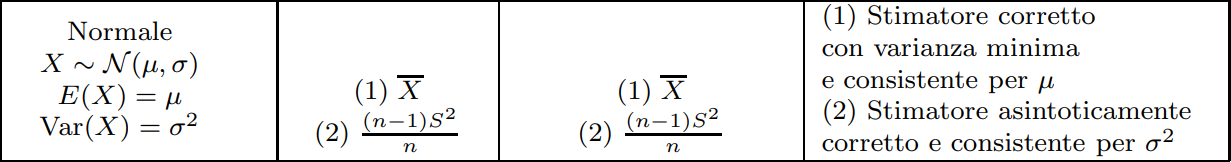
\includegraphics[height=2.2cm]{capitoli/images/2_stima_parametri/tabella.png}
\end{figure}
\vspace{5mm}

\section{Intervalli di confidenza}

Alla stima puntuale di un parametro non noto di una popolazione (costituita da un singolo valore reale) spesso si preferisce sostituire un intervallo di valori, detto \textbf{intervallo di confidenza} (o intervallo di fiducia), ossia si cerca di determinare in base ai dati del campione due limiti (uno inferiore e uno superiore) entro i quali sia compreso il parametro non noto con un certo \textbf{coefficiente di confidenza} (detto anche grado di fiducia).

\noindent \textbf{Definizione:} Fissato un coefficiente di confidenza $1-\alpha (0 < \alpha < 1)$, se è possibile scegliere le statistiche $\underline{C_n}$ e $\Bar{C_n}$ in modo tale che

\[P(\underline{C_n} < \theta < \Bar{C_n}) = 1 - \alpha\],

allora si dice che $(\underline{C_n}, \Bar{C_n})$ è un intervallo di confidenza di grado $1 - \alpha$ per $\theta$. Inoltre, le statistiche $\underline{C_n = g_1 = (X_1, X_2, ..., X_n)}$ e $\Bar{C_n} = g_2 = (X_1, X_2, ..., X_n)$ sono dette limite inferiore e superiore dell'intervallo di confidenza.

Se $g_1(x)$ e $g_2(x)$ sono i valori assunti dalle statistiche $\underline{C_n}$ e $\Bar{C_n}$ per il campione osservato $x = (x_1, x_2, ..., x_n)$, allora l'intervallo $(g_1(x), g_2(x))$ è detto stima dell'intervallo di confidenza di grado $1-\alpha$ per $\theta$ e i punti finali $g_1(x)$ e $g_2(x)$ di tale intervallo sono detti rispettivamente stima del limite inferiore e stima del limite superiore dell'intervallo di confidenza. La scelta dell'intervallo di confidenza deve essere effettuata in base ad alcune proprietà statistiche. Ad esempio, fissato un coefficiente di confidenza $1-\alpha$, alcune proprietà desiderabili sono che la lunghezza dell'intervallo di confidenza 

\[L(X_1, X_2, ..., X_n;1-\alpha) = \underline{C_n} - \Bar{C_n}\]

sia la più piccola possibile oppure che la lunghezza media di tale intervallo sia la più piccola possibile.

\subsection{Metodo Pivotale}

Un metodo per la costruzione degli intervalli di confidenza è il metodo pivotale. Tale metodo consiste essenzialmente nel determinare una variabile aleatoria di pivot $\gamma(X_1, X_2, ..., X_n;\theta)$ che dipende dal campione casuale $X_1, X_2, ..., X_n$ e dal parametro non noto $\theta$ e la cui funzione di distribuzione non contiene il parametro da stimare. Tale variabile aleatoria non è una statistica poiché dipende dal parametro non noto $\theta$ e quindi non è osservabile.

Sia $X_1, X_2, ..., X_n$ un campione casuale di ampiezza n estratto da una popolazione normale con valore medio $\mu$ e varianza $\delta^2$ si possono analizzare i seguenti problemi:

\begin{enumerate}
    \item determinare un intervallo di confidenza di grado $1 - \alpha$ per il valore medio $\mu$ nel caso in cui la varianza di $\delta^2$ della popolazione normale è nota;
    \item determinare un intervallo di confidenza di grado $1 - \alpha$ per il valore medio $\mu$ nel caso in cui la varianza della popolazione normale è non nota;
    \item determinare un intervallo di confidenza di grado $1 - \alpha$ per la varianza $\delta^2$ nel caso in cui il valore medio $\mu$ della popolazione normale è noto;
    \item determinare un intervallo di confidenza di grado $1 - \alpha$ per la varianza $\delta^2$ nel caso in cui il valore medio della popolazione normale è non noto.
\end{enumerate}

In questo lavoro ci focalizzeremo sul secondo e sul quarto problema.

\vspace{5mm}
\noindent \textbf{Intervallo di confidenza per $\mu$ con varianza non nota}

Per determinare un intervallo di confidenza di grado $1-\alpha$ per il valore medio $\mu$ nel caso in cui la varianza $\delta^2$ della popolazione normale non è nota, utilizziamo il metodo pivotale e consideriamo la variabile aleatoria di pivot:

\[T_n = \frac{\Bar{X_n} - \mu}{S_n/\sqrt{n}}\]

Tale variabile aleatoria dipende dal campione casuale e dal parametro non noto $\mu$. Inoltre, poiché:

\[T_n = \frac{\Bar{X} - \mu}{\delta / \sqrt{n}}\sqrt{\frac{\delta^2}{S_n^2}} = \frac{Z_n}{\sqrt{Q_n}/(n-1)}\]

si ha che $T_n$ è distribuita con legge di Student con $n-1$ gradi di libertà.

Scegliendo nel metodo pivotale $\alpha1 = -t_{\alpha/2,n-1}$ e $\alpha2 = t_{\alpha/2,n-1}$ dove $t_{\alpha/2,n-1}$ è tale che 

\[P(T_n < -t_{\alpha/2,n-1}) = P(T_n>t_{\alpha/2,n-1}) = \frac{\alpha}{2}\]

ne deriva che:

\[P(-t_{\alpha/2,n-1} < T_n < t_{\alpha/2,n-1}) = 1-\alpha\]

Dalla probabilità ottenuta si ottiene:

\[P(\Bar{X}_n - t_{\alpha/2,n-1} \frac{S_n}{\sqrt{n}} <\mu < \Bar{X}_n + t_{\alpha/2,n-1}\frac{S_n}{\sqrt{n}} = 1- \alpha\]

Se poniamo:

\[\underline{C_n} = \Bar{X}_n - t_{\alpha/2,n-1}\frac{S_n}{\sqrt{n}}, \Bar{C}_n = \Bar{X}_n + t_{\alpha/2,n-1}\frac{S_n}{\sqrt{n}}\]

si ha che $(\underline{C_n}, \Bar{C}_n)$ è un intervallo di confidenza di grado $1 - \alpha$ per $\mu$, dove le statistiche $(\underline{C_n}$ e $\Bar{C}_n)$ rappresentano il limite inferiore e superiore rispettivamente. Si può ora definire la lunghezza dell'intervallo di confidenza:

\[L(X_1, X_2, ..., X_n;1-\alpha) = \Bar{C}_n - \underline{C_n} = 2t_{\alpha/2,n-1}\frac{S_n}{\sqrt{n}}\]

Quindi, per ogni fissato campione osservato $(x_1, x_2, ..., x_n)$ a valori sempre più piccoli di $\alpha$, corrispondono lunghezze di intervalli di confidenza sempre più ampi. Da tutto ciò ne deriva che dato un campione $(x_1, x_2, ..., x_n)$ di ampiezza n estratto da una popolazione normale con varianza non nota si ha che la stima dell'intervallo di confidenza di grado $1-\alpha$ per il valore medio $\mu$ è 

\[\Bar{x}_n = t_{\alpha/2,n-1}\frac{S_n}{\sqrt{n}} < \mu < \Bar{x}_n + t_{\alpha/2,n-1}\frac{S_n}{\sqrt{n}}\]

dove $x_n$ e $S_n$ denotano rispettivamente la media e la deviazione standard campionaria delle n osservazioni.

\vspace{5mm}
\noindent \textbf{Metodo pivotale - applicazione}

Si considerino 2 casi in particolare:

\begin{itemize}
    \item $\alpha = 0.05$
    \item $\alpha = 0.01$
\end{itemize}

\vspace{5mm}
\noindent \textbf{Stima dell'intervallo di confidenza di grado $1 - \alpha = 0.95$}

\begin{lstlisting}
  alpha <- 1 - 0.95
  n <- length(ds)
  mean(ds)
  [1] 1.996316
  sd(ds)
  [1] 0.51082
  mean(ds) - qt(1 - alpha / 2, df = n - 1) * sd(ds) / sqrt(n)
  [1] 1.882638
  mean(ds) + qt(1 - alpha / 2, df = n - 1) * sd(ds) / sqrt(n)
  [1] 2.109993
\end{lstlisting}

La stima dell'intervallo di confidenza di grado $1-\alpha = 0.95$ per il quantitativo medio è (1.88, 2.11), ed è osservabile come $\mu$ sia compreso nell'intervallo.

\vspace{5mm}
\noindent \textbf{Stima dell'intervallo di confidenza di grado $1 - \alpha = 0.99$}

\begin{lstlisting}
  alpha <- 1 - 0.99
  n <- length(ds)
  mean(ds)
  [1] 1.996316
  sd(ds)
  [1] 0.51082
  mean(ds) - qt(1 - alpha / 2, df = n - 1) * sd(ds) / sqrt(n)
  [1] 1.84557
  mean(ds) + qt(1 - alpha / 2, df = n - 1) * sd(ds) / sqrt(n)
  [1] 2.147062
\end{lstlisting}

La stima dell'intervallo di confidenza di grado $1-\alpha = 0.5$ per il quantitativo medio è (1.85, 2.15), ed è osservabile come $\mu$ sia compreso nell'intervallo.

Si nota che aumentando il grado di fiducia, aumenta anche la lunghezza dell'intervallo di confidenza.

\vspace{5mm}
\noindent \textbf{Intervallo di confidenza per $\delta^2$ con valore medio non noto}

Per determinare un intervallo di confidenza di grado $1-\alpha$ per la varianza $\delta^2$ nel caso in cui il valore medio $\mu$ della popolazione non è noto, utilizziamo il metodo pivotale e consideriamo la variabile aleatoria di pivot:

\[Q_n = \frac{(n-1)S_n^2}{\delta^2} = \frac{1}{\delta^2}\sum_{i=1}^n(X_i - \Bar{X}_n)^2\]

Tale variabile aleatoria dipende dal campione casuale e dal parametro non noto $\delta^2$ ed è distribuita con legge chi-quadrato con n-1 gradi di libertà.

Scegliendo nel metodo pivotale $\alpha_1 = X^2_{1-\alpha/2,n-1}$ e $\alpha_2 = X^2_{\alpha/2,n-1}$ ina maniera tale che

\[P(0<Q_n<X^2_{1-\alpha/2,n-1} = P(Q_n>X^2_{\alpha/2,n-1} = \frac{\alpha}{2}\]

ne deriva che:

\[P(X^2_{1-\alpha/2,n-1} < Q_n < X^2_{\alpha/2,n-1}) = 1-\alpha\]

Dalla probabilità ottenuta abbiamo:

\[P(X^2_{1-\alpha/2,n-1} < \frac{(n-1)S_n^2}{\delta^2}<X^2_{\alpha/2,n-1} = 1-\alpha\]

che è equivalente a richiedere che 

\[P(\frac{(n-1)S_n^2}{X^2_{\alpha/2,n-1}} < \delta^2 < \frac{(n-1)S^2_n}{X^2_{1-\alpha/2,n-1}}) = 1-\alpha\]

Se poniamo

\[\underline{C_n} = \frac{(n-1)S_n^2}{X^2_{\alpha/2,n-1}}, \quad \Bar{X}_n = \frac{(n-1)S^2_n}{X^2_{1-\alpha/2,n-1}}\]

si ha che $(\underline{C_n}, \Bar{C}_n)$ è un intervallo di confidenza di grado $1-\alpha$ per $\delta^2$, dove le statistiche $\underline{C_n}$ e $\Bar{C}_n$ rappresentano il limite inferiore e superiore rispettivamente. Quindi, per ogni fissato campione osservato $(x_1, x_2, ..., x_n)$, a valori sempre più piccoli di $\alpha$ corrispondono lunghezze di intervalli di confidenza sempre più ampi. Da tutto ciò ne deriva che, dato un campione $(x_1, x_2, ..., x_n)$ di ampiezza n estratto da una popolazione normale con valore medio non noto si ha che la stima dell'intervallo di confidenza di grado $1-\alpha$ per la  varianza $\delta^2$ è

\[\frac{(n-1)S_n^2}{X^2_{\alpha/2,n-1}} < \delta^2 < \frac{(n-1)S^2_n}{X^2_{1-\alpha/2,n-1}}\]

dove

\[s_n^2 = \frac{1}{n-1} \sum_{i+1}^n (x_i - \Bar{x})n)^2\]

denota la varianza campionaria delle n osservazioni.

\vspace{5mm}
\noindent \textbf{Metodo pivotale - applicazione}

Si considerino 2 casi in particolare:

\begin{itemize}
    \item $\alpha = 0.05$
    \item $\alpha = 0.01$
\end{itemize}

\vspace{5mm}
\noindent \textbf{Stima dell'intervallo di confidenza di grado $1 - \alpha = 0.95$}

\begin{lstlisting}
 alpha <- 1 - 0.95
 n <- length(ds)
 var(ds)
 [1] 0.2609371
 (n-1)*var(ds)/qchisq(1-alpha/2,df=n-1)
 [1] 0.1954441
 (n-1)*var(ds)/qchisq(alpha/2,df=n-1)
 [1] 0.3660883
\end{lstlisting}

La stima dell'intervallo di confidenza di grado $1-\alpha = 0.5$ per la varianza è (0.195, 0.366) ed è osservabile come $\delta^2$ sia compreso in questo intervallo.

\vspace{5mm}
\noindent \textbf{Stima dell'intervallo di confidenza di grado $1 - \alpha = 0.99$}

\vspace{5mm}
\begin{lstlisting}
 alpha <- 1 - 0.99
 n <- length(ds)
 var(ds)
 [1] 0.2609371
 (n-1)*var(ds)/qchisq(1-alpha/2,df=n-1)
 [1] 0.1790709
 (n-1)*var(ds)/qchisq(alpha/2,df=n-1)
 [1] 0.4092025
\end{lstlisting}

La stima dell'intervallo di confidenza di grado $1-\alpha = 0.5$ per la varianza è (0.179, 0.409) ed è osservabile come $\delta^2$ sia compreso in questo intervallo.

Si nota che aumentando il grado di fiducia, aumenta la lunghezza dell'intervallo di confidenza.

Per una popolazione normale, le stime per intervallo del valore $\mu$ e della varianza $\delta^2$ della popolazione possono essere effettuate qualsiasi sia la dimensione del campione casuale osservato. Ciò dipende dalla circostanza favorevole di conoscere la distribuzione esatta della variabile pivotale considerata: normale e di Student per la stima del valore medio e chi-quadrato per la stima della varianza.
%################################################

\newpage
\phantomsection
\definecolor{dkgreen}{rgb}{0,0.6,0}
\definecolor{gray}{rgb}{0.5,0.5,0.5}
\definecolor{mauve}{rgb}{0.58,0,0.82}

\lstset{frame=tb,
language=R,
aboveskip=3mm,
belowskip=3mm,
showstringspaces=false,
columns=flexible,
numbers=none,
inputencoding=utf8/latin1,
keywordstyle=\color{blue},
numberstyle=\tiny\color{gray},
commentstyle=\color{dkgreen},
stringstyle=\color{mauve},
breaklines=true,
breakatwhitespace=true,
tabsize=3
}

\chapter{Verifica delle ipotesi}

\section{Introduzione}

Dopo la stima dei parametri il passo successivo è la verifica delle ipotesi. La verifica delle ipotesi interviene ogni volta che si ha il bisogno di predire qualcosa, come ad esempio nelle indagini sperimentali.

In generale gli elementi che costituiscono il punto di partenza del procedimento di verifica delle ipotesi sono una popolazione descritta da una variabile aleatoria X caratterizzata da una funzione di probabilità o densità di probabilità $f(x;\theta)$, un'ipotesi su di un parametro non noto della popolazione ed un campione casuale $X_1, X_2, ..., X_n$ estratto dalla popolazione. Si può ora definire il concetto di ipotesi statistica.

\noindent \textbf{Definizione:} Un'ipotesi statistica è un'affermazione o una congettura sul parametro non noto $\theta$. Se l'ipotesi statistica specifica completamente $f(x;\theta)$ è detta ipotesi semplice, altrimenti è chiamata ipotesi composta.

\noindent \textbf{Esempio:} Sia $X_1, X_2, ..., X_n$ un campione casuale estratto da una popolazione normale con varianza nota $\delta^2$. Allora, l'ipotesi statistica $H: \mu = 1400$ è semplice poiché, essendo nota la varianza, specifica completamente la densità, mentre l'ipotesi $H: \mu \leq 1400$ è composta poiché non specifica completamente la densità. Se invece la varianza della popolazione normale non è nota, l'ipotesi statistica $H:\mu = 1400$ diventa composta poiché, essendo $\delta^2$ non nota, essa non specifica completamente la densità.

L'ipotesi soggetta a verifica viene in genere denotata con $H_0$ e viene chiamata \textbf{\textit{ipotesi nulla}}. Si chiama \textbf{test di ipotesi $\phi$} il procedimento o regola con cui si decide, sulla base dei dati del campione, se accettare o rifiutare $H_0$. La costruzione del test richiede la formulazione, in contrapposizione all'ipotesi nulla, di una proposizione alternativa. Questa proposizione prende il nome di \textbf{ipotesi alternativa} indicata con $H_1$. L'ipotesi nulla, cioè l'ipotesi soggetta a verifica, si ha quindi $\theta \in \Theta_0$ e l'ipotesi alternativa si ha quando $\theta \in \Theta_1$ e si scrive

\[H_0:\theta \in \Theta_0, \quad H_1: \theta \in \Theta_1,\]

avendo denotato con $\Theta_0$ e $\Theta_1$ due sottoinsiemi disgiunti dello spazio $\Theta$ dei parametri.

L'obiettivo è determinare un test $\phi$ che permetta di suddividere l'insieme dei campioni in due sottoinsiemi:

\begin{itemize}
    \item una regione di accettazione A,
    \item una di rifiuto R
\end{itemize}

dell'ipotesi nulla.
In generale si può incorrere in due tipi di errore

\begin{itemize}
    \item Tipo 1: rifiutare l'ipotesi nulla $H_0$ nel caso in cui tale ipotesi sia vera, denotato con 

    \[\alpha(\theta) = P(rifiutare H_0 | \theta), \quad \theta \in \Theta_0\]

    \item Tipo 2: accettare l'ipotesi nulla $H_0$ nel caso in cui tale ipotesi sia falsa, denotato con 

    \[\beta(\theta) = P(accettare H_0|\theta), \quad \theta \in \Theta_1\]
\end{itemize}

\vspace{5mm}
\begin{tabular}{c|c|c}
 & Rifiutare $H_0$ & Accettare $H_0$ \\
 $H_0$ vera & Errore del 1 tipo, probabilità $\alpha$ & Decisione esatta, probabilità $1-\alpha$ \\
 $H_0$ falsa & Decisione esatta, probabilità $1-\beta$ & Errore del 2 tipo, probabilità $\beta$
\end{tabular}
\vspace{5mm}

Un concetto importante è quello di \textbf{\textit{misura della regione critica}}.

La misura della regione critica di un test fornisce la probabilità massima di commettere un errore del 1 tipo al variare di $\theta \in \Theta_0$, ossia la probabilità massima di rifiutare l'ipotesi nulla quando essa è vera e si indica con

\[\alpha = sup_{\theta \in \Theta_0} \alpha(\theta)\]

In generale per campioni casuali di fissata ampiezza, se si diminuisce la probabilità di commettere un errore di tipo 1 aumenta la probabilità di commettere un errore di tipo 2 e viceversa. Di solito, si scelgono le ipotesi in modo da rendere l'errore di tipo 1 più grave in modo da imporre che la probabilità di commettere tale errore sia piccola. Nella costruzione del test set conviene quindi fissare la probabilità di commettere un errore di tipo 1 e cercare un test $\phi$ che minimizzi la probabilità di commettere un errore di tipo 2.

Solitamente la probabilità di commettere un errore di tipo 1 si sceglie uguale a 

\begin{itemize}
    \item 0.05, test statisticamente significativo
    \item 0.01, test statisticamente molto significativo
    \item 0.001 test statisticamente estremamente significativo
\end{itemize}

Si noti che quanto minore è il valore di $\alpha$ tanto maggiore è la credibilità di un eventuale rifiuto dell'ipotesi nulla.

I test statistici sono di due tipi: test unilaterali (detti anche unidirezionali) e test bilaterali (detti anche bidirezionali). Un test bilaterale è il seguente

\[H_0:\theta=\theta_0\]
\[H_1:\theta \neq \theta_0\]

mentre gli unilaterali sono:

\[H_0:\theta \leq \theta_0 \quad H_0:\theta \geq \theta_0\]
\[H_1:\theta > \theta_0 \quad H_1:\theta < \theta_0\]

\subsection{Test su Popolazione Normale}

In questo paragrafo si effettua la verifica delle ipotesi sul valore medio $\mu$ nel caso in cui la varianza $\delta^2$ della popolazione normale è non nota e sulla varianza $\delta^2$ nel caso in cui il valore medio $\mu$ della popolazione normale non è noto.

\vspace{5mm}
\noindent \textbf{p-value}

Nella statistica inferenziale il valore \textbf{p} (o p-value) di un test di verifica d'ipotesi indica la probabilità di ottenere un risultato uguale o "più estremo" di quello osservato, supposta vera l'ipotesi nulla. Talvolta viene anche chiamato \textbf{livello di significatività osservato}. Non dipende da $\alpha$ ma dal campione e dalla popolazione da cui è stato estratto il campione. Poiché le conclusioni dei test statistici dipendono dal livello di significatività $\alpha$, piuttosto che scegliere preventivamente un livello al quale verificare $H_0$, spesso si preferisce calcolare il p-value. Calcolando il p-value relativo ai dati osservati è possibile comportarsi come segue:

\begin{itemize}
    \item p > $\alpha$, l'ipotesi $H_0$ non può essere rifiutata;
    \item p $\leq$ $\alpha$, l'ipotesi $H_0$ deve essere rifiutata
\end{itemize}

Sia H l'ipotesi che il valore x dei dati osservati sia estratto da una certa variabile aleatoria X nota. Il p-value è definito come la probabilità, supposta l'ipotesi $H$, di ottenere un risultato (dai dati osservati) uguale o "più estremo" di quello effettivamente osservato. Il p-value è dato da:

\begin{itemize}
    \item $Pr(X \geq x|H)$ per test unilaterali destri;
    \item $Pr(X \leq x|H)$ per test unilaterali sinistri;
    \item $2 min\{Pr(X \leq x|H), Pr(X \geq x|H)\}$ per test bilaterali
\end{itemize}

\vspace{5mm}
\noindent \textbf{Test sul valore medio $\mu$ con varianza $\delta^2$ non nota}

Nelle prossime righe verrà analizzato il \textbf{test bilaterale}.

Sia $x_1, x_2, ..., x_n$ un campione casuale estratto da una popolazione normale con varianza non nota $\delta^2$. Si considerino le ipotesi:

\[H_0: \mu = \mu_0 \quad H_1:\mu \neq \mu_0\]

Essendo la varianza non nota, entrambe le ipotesi sono composte. Quando $H_0$ è vera, in analogia a quanto visto per gli intervalli di confidenza la variabile aleatoria diventa fondamentale:

\[T_n = \frac{\Bar{X}_n - \mu_0}{S_n/ \sqrt{n}}\]

che è distribuita con legge di Student con n-1 gradi di libertà. Il test bilaterale $\phi$ di misura $\alpha$ per le ipotesi $H_0$ e $H_1$ è il seguente:

\begin{itemize}
    \item si accetti $H_0$ se 
    \[-t_{\alpha/2, n-1} < \frac{\Bar{x}_n - \mu_0}{S_n/\sqrt{n}}<t_{\alpha/2, n-1}\]
    \item si rifiuti se
    \[\frac{\Bar{x}-\mu_0}{S_n/\sqrt{n}}<-t_{\alpha/2, n-1}\]

    oppure

    \[\frac{\Bar{x}-\mu_0}{S_n/\sqrt{n}}<t_{\alpha/2, n-1}\]
\end{itemize}

Si può ora applicare il test sul dataset precedentemente generato.

%test bilaterale
\vspace{5mm}
\noindent \textbf{Test statisticamente molto significativo}

Nel primo test si utilizza un livello di significatività pari all'1\%, con parametri: $H_0: \mu = 1.90$ e ipotesi alternativa $H_1: \mu \neq 1.90$. Nel caso considerato si ha dunque $\mu_0 = 1.90, \alpha = 0.01, n = 80, \Bar{x_{80}} = 1.996$ e $s_{80} = 0.510$.

\vspace{5mm}
\begin{lstlisting}
  alpha <- 0.01
  mu0 <- 1.90
  n <- length(ds)
  t_apha_m_01 <- qt(1 - alpha / 2, df = n - 1)
  t_apha_m_01
  [1] 2.639505

  meancamp <- mean(ds)
  devcamp <- sd(ds)
  t_01 <-(meancamp-mu0)/(devcamp/sqrt(n))
  t_01
  [1] 1.686455
\end{lstlisting}

\begin{figure}[!htb]
    \centering
    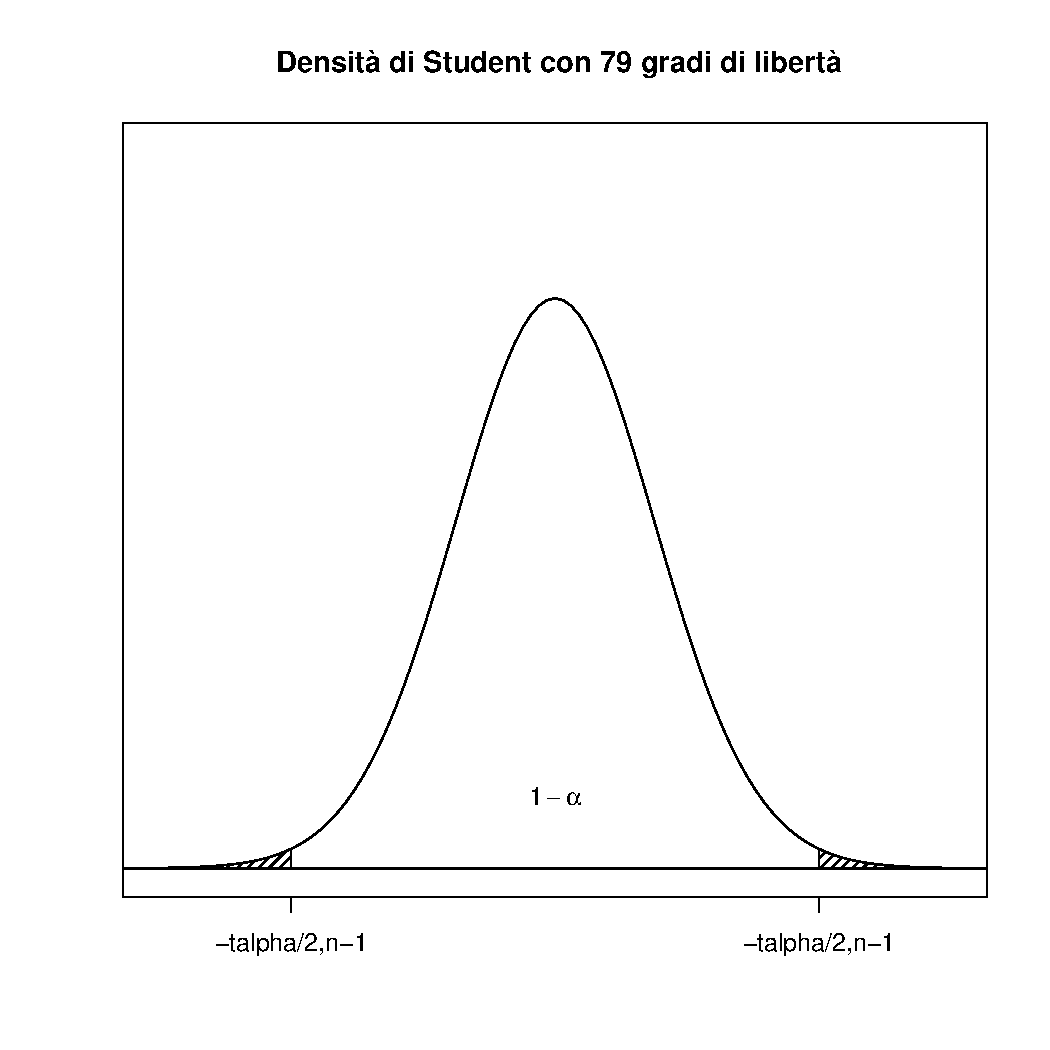
\includegraphics[height=16cm]{capitoli/images/3_verifica_ipotesi/curvehp1.pdf}
    \caption{Curva test bilaterale ipotesi 1}
\end{figure}

Dai risultati ottenuti si ha che l’ipotesi rientra nella regione di accettazione e quindi l’ipotesi $H_0$ viene accettata.

\vspace{5mm}
\noindent \textbf{Confronto con p-value}

\[pvalue = P(Z_n < -|z+{os}|) + P(Z_n > |z_{os}|) = 2P(Z_n>|z_{os}|) = 2[1-P(Z_n \leq |z_{os})],\]

\[dove \quad z_{os} = (\Bar{x}_n - \mu_0)/(\delta/\sqrt{n})\]

\begin{lstlisting}
  az <- abs(t_01)
  pvalue <- 2 * (1 - pnorm(az, mean = 0, sd = 1))
  pvalue
  [1] 0.09170812
\end{lstlisting}

Siccome $p \geq \alpha$, l'ipotesi $H_0$ viene accettata.

\vspace{5mm}
\noindent \textbf{Test statisticamente significativo}

Nel secondo test si utilizza un livello di significatività pari al 5\%, con parametri: $H_0$: $\mu = 1.90$ e ipotesi alternativa $H_1: \mu \neq 1.90$. Nel caso considerato si ha dunque $\mu_0 = 1.90, \alpha = 0.05, n = 80, \Bar{x_{80}} = 1.996$ e $s_{80} = 0.510$.

\vspace{5mm}
\begin{lstlisting}
  alpha <- 0.05
  mu0 <- 1.90
  n <- length(ds)
  t_apha_m_05 <- qt(1 - alpha / 2, df = n - 1)
  meancamp <- mean(ds)
  devcamp <- sd(ds)
  t_05 <- (meancamp - mu0) / (devcamp / sqrt(n))
  t_apha_m_05
  [1] 1.99045
  t_05
  [1] 1.686455
\end{lstlisting}

Dai risultati ottenuti si ha che l’ipotesi rientra nella regione di accettazione e quindi l’ipotesi $H_0$ viene accettata.

Nelle prossime righe si analizza il \textbf{test unilaterale sinistro}.

Sia $x_1, x_2, ..., x_n$ un campione casuale estratto da una popolazione normale con varianza non nota $\delta^2$. Si considerino le ipotesi:

\[H_0:\mu \leq \mu_0 \quad H_1:\mu > \mu_0\]

Entrambe le ipotesi $H_0$ e $H_1$ sono composte. Il test unilaterale sinistro $\psi$ di misura $\alpha$ per le ipotesi considerate è il seguente:

\begin{itemize}
    \item si accetti $H_0$ se $\frac{\Bar{x}_n - \mu_0}{s_n/\sqrt{n}} < t_{a,n-1}$
    \item si rifiuti $H_0$ se $\frac{\Bar{x}_n - \mu_0}{s_n/\sqrt{n}} > t_{a,n-1}$
\end{itemize}

Si può ora applicare il test sul dataset precedentemente generato.


%test unilaterale sinistro
\vspace{5mm}
\noindent \textbf{Test statisticamente molto significativo}

Nel primo test si utilizza un livello di significatività pari all'1\%, con parametri: $H_0$: $\mu \leq 4$ e ipotesi alternativa $H_1: \mu > 4$. Nel caso considerato si ha dunque $\mu_0 = 4, \alpha = 0.01, n = 80, \Bar{x_{80}} = 1.996$ e $s_{80} = 0.510$.

\vspace{5mm}
\begin{lstlisting}
  alpha <- 0.01
  mu0 <- 1
  n <- 80
  qt(1 - alpha, df = n - 1)
  [1] 2.374482
  
  meancamp <- mean(ds)
  devcamp <- sd(ds)
  t_01 <-(meancamp - mu0) / (devcamp / sqrt(n))
  [1] 17.44513
\end{lstlisting}

\begin{figure}[!htb]
    \centering
    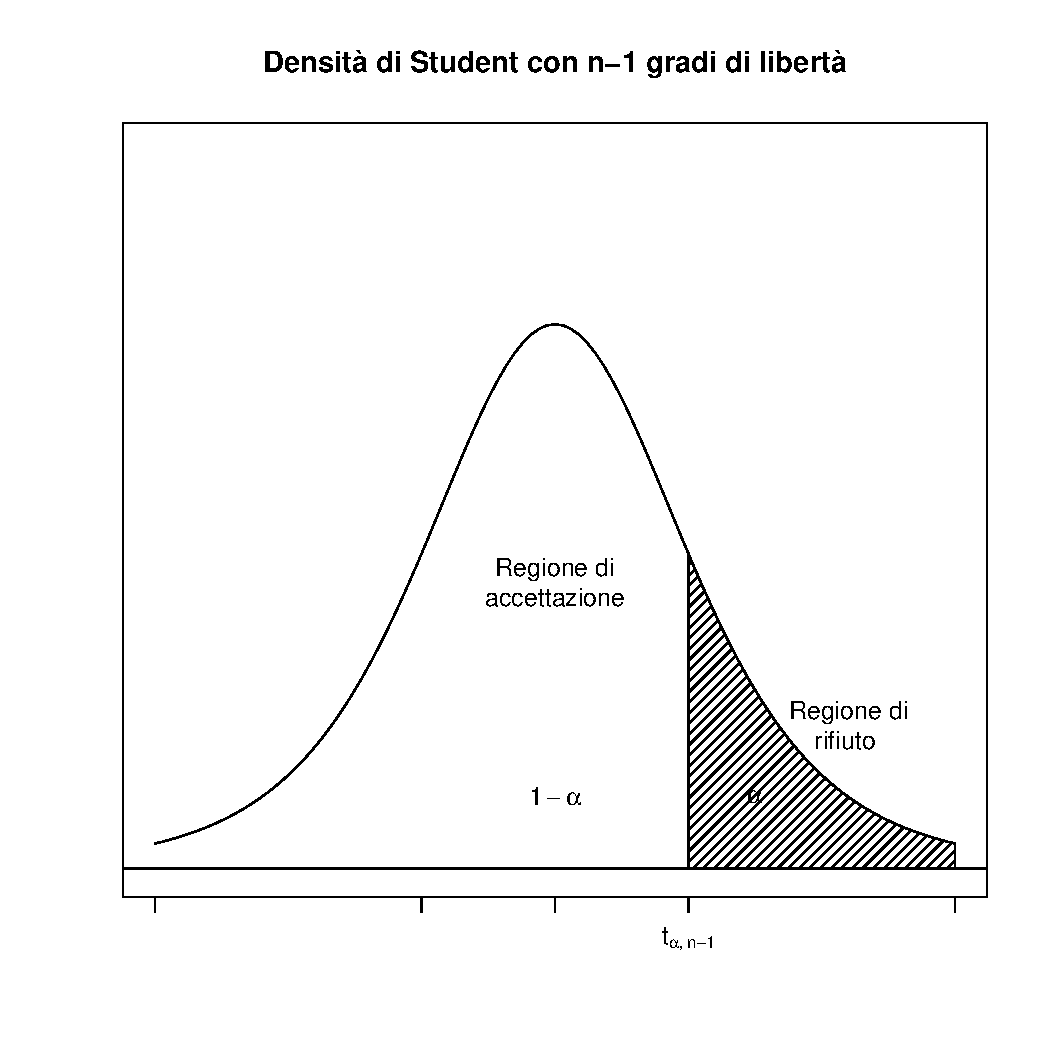
\includegraphics[height=16cm]{capitoli/images/3_verifica_ipotesi/curvehp3.pdf}
    \caption{Curva test unilaterale sinistro ipotesi 1}
\end{figure}

Dai risultati si ottiene che l'ipotesi non rientra nella regione di accettazione e quindi l'ipotesi $H_0$ viene rifiutata.

\vspace{5mm}
\noindent \textbf{Confronto con p-value}

\[pvalue = P(Z_n > z_{os}) = 1-P(Z_n \leq z_{os})\],

\[dove \quad z_{os} = (\Bar{x}_n - \mu_0)/(\delta/\sqrt{n})\]

\vspace{5mm}
\begin{lstlisting}
  z<-abs(t_01)
  pvalue <- 1 - pnorm(z, mean = 0, sd = 1)
  pvalue
  [1] 0
\end{lstlisting}

Siccome $p<\alpha$, l'ipotesi viene rifiutata.
 
\vspace{5mm}
\noindent \textbf{Test statisticamente significativo}

Nel secondo test si utilizza un livello di significatività pari al 5\%, con parametri: $H_0$: $\mu \leq 4$ e ipotesi alternativa $H_1: \mu > 4$. Nel caso considerato si ha dunque $\mu_0 = 4, \alpha = 0.05, n = 80, \Bar{x_{80}} = 1.996$ e $s_{80} = 0.510$.

\vspace{5mm}
\begin{lstlisting}
   alpha <-0.05
   mu0 <- 1
   n<- 80
   qt(1-alpha ,df=n-1)
   [1] 1.664371

   meancamp <- mean(ds)
   devcamp <- sd(ds)
   t_05 <- (meancamp - mu0) / (devcamp / sqrt(n))
   t_05
   [1] 17.44513
\end{lstlisting}

\vspace{5mm}
\begin{lstlisting}
  curve(dt(x, df = 5), from = -3, to = 3, axes = FALSE, ylim = c(0, 0.5)
    , xlab = "", ylab = "", main = "Densità di Student con n-1 gradi di libertà")
  text(0, 0.05, expression(1 - alpha))
  text(0, 0.2, "Regione di\naccettazione")
  axis(1, c(-3, -1, 0, 1, 3), c("", " ", " ", expression(t[list(alpha, n - 1)]), ""))
  vals <- seq(1, 3, length = 100)
  x <- c(1, vals, 3, 1)
  y <- c(0, dt(vals, , df = 5), 0, 0)
  polygon(x, y, density = 20, angle = 45)
  abline(h = 0)
  text(1.5, 0.05, expression(alpha))
  text(2.2, 0.1, "Regione di\nrifiuto ")
  box()
\end{lstlisting}

\begin{figure}[!htb]
    \centering
    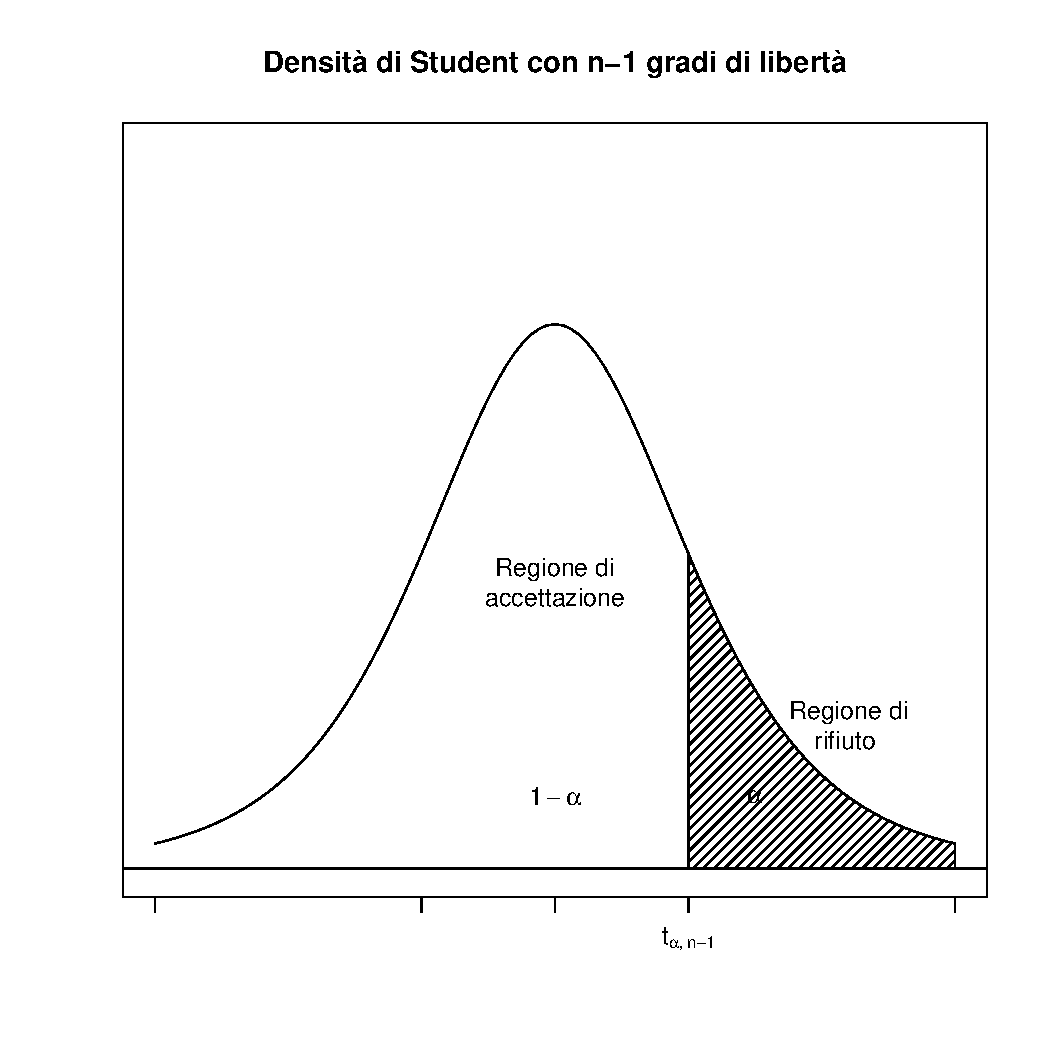
\includegraphics[height=16cm]{capitoli/images/3_verifica_ipotesi/curvehp4.pdf}
    \caption{Curva test unilaterale sinistro ipotesi 2}
\end{figure}

Dai risultati ottenuti si ha che l'ipotesi non rientra nella regione di accettazione e quindi l'ipotesi $H_0$ viene rifiutata.

Nelle prossime righe si analizza il \textbf{test unilaterale destro.}

Sia $x_1, x_2, ..., x_n$ un campione casuale estratto da una popolazione normale con varianza non nota $\delta^2$. Si considerino le ipotesi:

\[H_0:\mu \geq \mu_0 \quad H_1:\mu < \mu_0\]

Il test unilaterale destro $\psi$ di misura $\alpha$ per le ipotesi considerate è il seguente:

\begin{itemize}
    \item si accetti $H_0$ se $\frac{\Bar{x}_n - \mu_0}{s_n/\sqrt{n}} > -t_{a,n-1}$
    \item si rifiuti $H_0$ se $\frac{\Bar{x}_n - \mu_0}{s_n/\sqrt{n}} < -t_{a,n-1}$
\end{itemize}

Si può ora applicare il test sul dataset precedentemente generato

%test unilaterale destro
\vspace{5mm}
\noindent \textbf{Test statisticamente molto significativo}

Nel primo test si utilizza un livello di significatività pari all'1\%, con parametri: $H_0$: $\mu \geq 3$ e ipotesi alternativa $H_1: \mu < 3$. Nel caso considerato si ha dunque $\mu_0 = 3, \alpha = 0.01, n = 80, \Bar{x_{80}} = 1.996$ e $s_{80} = 0.510$.

\vspace{5mm}
\begin{lstlisting}
    alpha <-0.01
    mu0<-3
    n<-length(ds)
    qt(alpha ,df=n-1)
    [1] -2.374482

    meancamp <- mean(ds)
    devcamp <- sd(ds)
    t_01 <- (meancamp - mu0) / (devcamp / sqrt(n))
    t_01
    [1] -17.57414
\end{lstlisting}

\vspace{5mm}
\begin{lstlisting}
  curve(dt(x, df = n - 1), from = -3, to = 3, axes = FALSE, ylim = c(0, 0.5)
    , xlab = "", ylab = "", main = paste("Densità di Student con n-1 gradi di libertà"))
  text(0, 0.05, expression(1 - alpha))
  text(0, 0.2, "Regione di\naccettazione")
  axis(1, c(-3, -1, 0, 1, 3), c("", expression(-t[list(alpha, n - 1)]), " ", " ", ""))
  vals <- seq(-3, -1, length = 100)
  x <- c(-3, vals, -1, -3)
  y <- c(0, dt(vals, , df = 5), 0, 0)
  polygon(x, y, density = 20, angle = 45)
  abline(h = 0)
  text(-1.5, 0.05, expression(alpha))
  text(-2.2, 0.1, "Regione di\nrifiuto")
  box()
\end{lstlisting}

\begin{figure}[!htb]
    \centering
    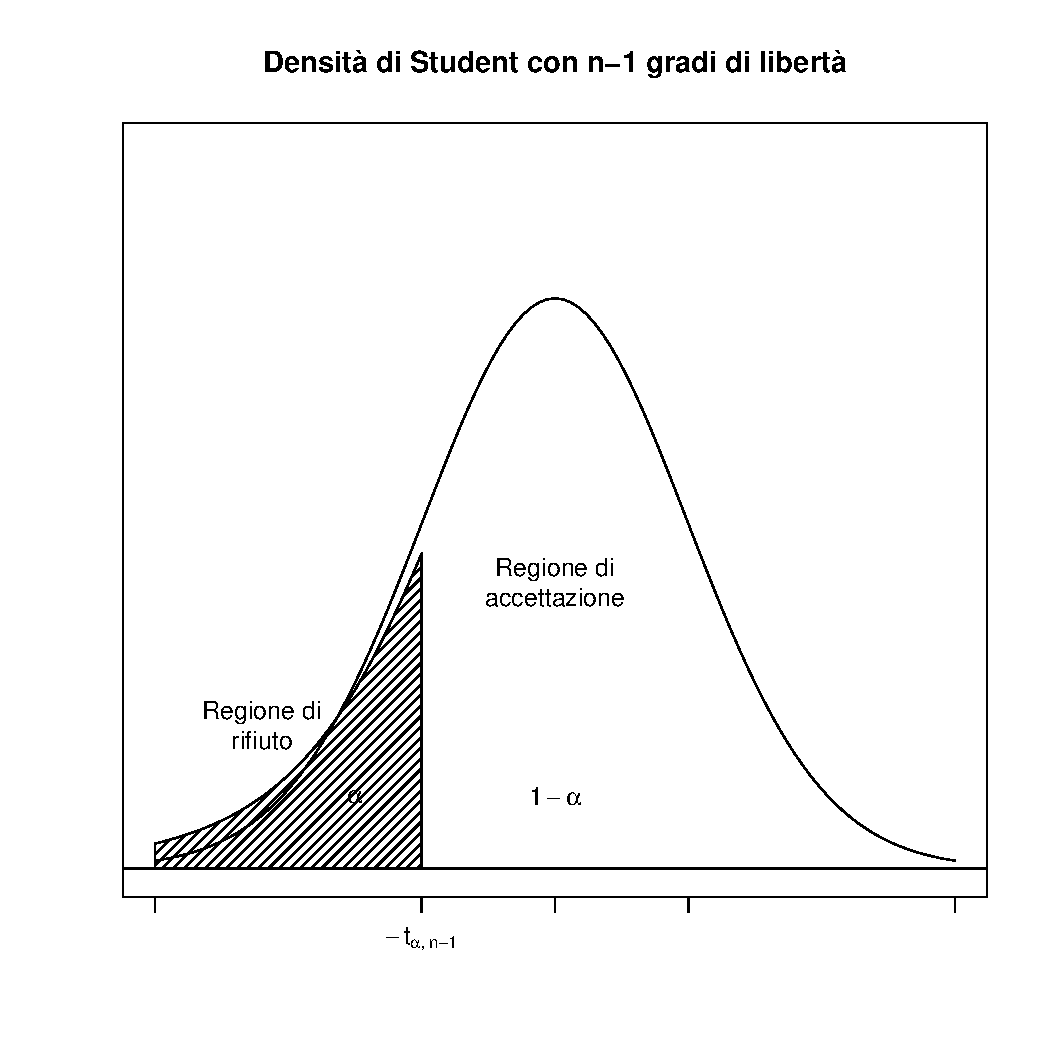
\includegraphics[height=16cm]{capitoli/images/3_verifica_ipotesi/curvehp5.pdf}
    \caption{Curva test unilaterale destro ipotesi 1}
\end{figure}

Dai risultati ottenuti si ha che l'ipotesi non rientra nella regione di accettazione e quindi l'ipotesi $H_0$ viene rifiutata.

\vspace{5mm}
\noindent \textbf{Confronto con p-value}

\[pvalue = P(Z_n \leq z_{os})\],

\[dove \quad z_{os} = (\Bar{x}_n - \mu_0)/(\delta/\sqrt{n})\]

\vspace{5mm}
\begin{lstlisting}
  z<-abs(t_01)
  pvalue <- 1 - pnorm(z, mean = 0, sd = 1)
  pvalue
  [1] 0
\end{lstlisting}

Siccome $p < \alpha$, rifiuto l'ipotesi.

\vspace{5mm}
\noindent \textbf{Test statisticamente significativo}

Nel secondo test si utilizza un livello di significatività pari al 5\%, con parametri: $H_0$: $\mu \geq 3$ e ipotesi alternativa $H_1: \mu < 3$. Nel caso considerato si ha dunque $\mu_0 = 3, \alpha = 0.05, n = 80, \Bar{x_{80}} = 1.996$ e $s_{80} = 0.510$.


\vspace{5mm}
\begin{lstlisting}
    alpha <-0.05
    mu0<-3
    n<-length(ds)
    qt(alpha ,df=n-1)
    [1] -1.664371

    meancamp <- mean(ds)
    devcamp <- sd(ds)
    t_05 <- (meancamp - mu0) / (devcamp / sqrt(n))
    t_05
    [1] -17.57414
\end{lstlisting}

\vspace{5mm}
\begin{lstlisting}
  curve(dt(x, df = n - 1), from = -3, to = 3, axes = FALSE, ylim = c(0, 0.5)
    , xlab = "", ylab = "", main = paste("Densità di Student con n-1 gradi di libertà"))
  text(0, 0.05, expression(1 - alpha))
  text(0, 0.2, "Regione di\naccettazione")
  axis(1, c(-3, -1, 0, 1, 3), c("", expression(-t[list(alpha, n - 1)]), " ", " ", ""))
  vals <- seq(-3, -1, length = 100)
  x <- c(-3, vals, -1, -3)
  y <- c(0, dt(vals, , df = 5), 0, 0)
  polygon(x, y, density = 20, angle = 45)
  abline(h = 0)
  text(-1.5, 0.05, expression(alpha))
  text(-2.2, 0.1, "Regione di\nrifiuto")
  box()
\end{lstlisting}

Dai risultati ottenuti si ha che l'ipotesi non rientra nella regione di accettazione e quindi l'ipotesi $H_0$ viene rifiutata.

\vspace{5mm}
\noindent \textbf{Test su $\delta^2$ con valore medio $\mu$ non noto}

Nelle prossime righe si analizza il \textbf{test bilaterale.}

Sia $x_1, x_2, ..., x_n$ un campione casuale estratto da una popolazione normale con valore medio non noto $\mu$. Si considerino le ipotesi:

\[H_0:\delta^2 = \delta^2_0 \quad H_0:\delta^2 \neq \delta^2_0\]

Entrambe le ipotesi sono composte. Quando l'ipotesi $H_0$ è vera, gioca un ruolo rilevante la variabile aleatoria

\[Q_n = \frac{(n-1)S_n^2}{\delta^2} = \frac{1}{\delta^2} \sum_{i=1}^n(X_i - X_n)^2\]

che è distribuita con legge chi-quadrato con n-1 gradi di libertà.

Il test bilaterale $\psi$ di misura $\alpha$ per le ipotesi considerate è:

\begin{itemize}
    \item si rifiuti $H_0$ se $\frac{(n-1)S_n^2}{\delta_0^2} < \chi_{1-\alpha/2,n-1}^2$ oppure $\frac{(n-1)S_n^2}{\delta_0^2} > \chi_{\alpha/2,n-1}^2$
    \item si accetti $H_0$ se $\chi_{1-\alpha/2,n-1}^2 < \frac{(n-1)S_n^2}{\delta_0^2} < \chi_{\alpha/2,n-1}^2$
\end{itemize}

Si può ora applicare il test sul dataset precedentemente generato.

%test bilterale
\vspace{5mm}
\noindent \textbf{Test statisticamente molto significativo}

Nel primo test si utilizza un livello di significatività pari all'1\%, con parametri: $H_0$: $\delta^2 = 1$ e ipotesi alternativa $H_1: \delta^2 \neq 1$. Nel caso considerato si ha dunque $\mu_0 = 1, \alpha = 0.01, n = 80,$ e $s_{80}^2 = 0.260$.

\vspace{5mm}
\begin{lstlisting}
  alpha <- 0.01
  sigma02 <- 1
  n <- length(ds)
  varcamp <- 0.260
  qchisq(alpha / 2, df = n - 1)
  [1] 50.37612
  qchisq(1 - alpha / 2, df = n - 1)
  [1] 115.1166
  (n-1)*varcamp /sigma02
  [1] 20.54
\end{lstlisting}

Dai risultati ottenuti si ha che l'ipotesi non rientra nella regione di accettazione e quindi l'ipotesi $H_0$ viene rifiutata.

\vspace{5mm}
\noindent \textbf{Test statisticamente significativo}

Nel secondo test si utilizza un livello di significatività pari al 5\%, con parametri: $H_0$: $\delta^2 = 1$ e ipotesi alternativa $H_1: \delta^2 \neq 1$. Nel caso considerato si ha dunque $\mu_0 = 1, \alpha = 0.05, n = 80$ e $s_{80}^2 = 0.260$.

\vspace{5mm}
\begin{lstlisting}
  alpha <- 0.05
  sigma02 <- 1
  n <- length(ds)
  varcamp <- 0.260
  qchisq(alpha / 2, df = n - 1)
  [1] 56.3089
  qchisq(1 - alpha / 2, df = n - 1)
  [1] 105.4728
  (n - 1) * varcamp / sigma02
  [1] 20.54
  
\end{lstlisting}

Dai risultati ottenuti si ha che l'ipotesi non rientra nella regione di accettazione e quindi l'ipotesi $H_0$ viene rifiutata.

Nelle prossime righe si analizza il \textbf{test unilaterale sinistro}.

Sia $x_1, x_2, ..., x_n$ un campione casuale estratto da una popolazione normale con valore medio non noto $\mu$. Si considerino le ipotesi:

\[H_0:\delta^2 \leq \delta^2_0 \quad H_0:\delta^2 > \delta^2_0\]

Entrambe le ipotesi sono composte. Quando l'ipotesi $H_0$ è vera, gioca un ruolo rilevante la variabile aleatoria

\[Q_n = \frac{(n-1)S_n^2}{\delta^2} = \frac{1}{\delta^2} \sum_{i=1}^n(X_i - X_n)^2\]

Il test bilaterale $\psi$ di misura $\alpha$ per le ipotesi considerate è: 

\begin{itemize}
    \item Si rifiuti $H_0$ se $\frac{(n-1)S_n^2}{\delta_0^2} > \chi_{\alpha/2,n-1}^2$
    \item Si accetti $H_0$ se $\frac{(n-1)S_n^2}{\delta_0^2} < \chi_{\alpha/2,n-1}^2$
\end{itemize}

Nelle prossime righe analizzeremo il \textbf{test unilaterale destro.}

Sia $x_1, x_2, ..., x_n$ un campione casuale estratto da una popolazione normale con valore medio non noto $\mu$. Si considerino le ipotesi:

\[H_0:\delta^2 \geq \delta^2_0 \quad H_0:\delta^2 < \delta^2_0\]

Entrambe le ipotesi sono composte. Quando l'ipotesi $H_0$ è vera, gioca un ruolo rilevante la variabile aleatoria

\[Q_n = \frac{(n-1)S_n^2}{\delta^2} = \frac{1}{\delta^2} \sum_{i=1}^n(X_i - X_n)^2\]

Il test bilaterale $\psi$ di misura $\alpha$ per le ipotesi considerate è: 

\begin{itemize}
    \item Si rifiuti $H_0$ se $\frac{(n-1)S_n^2}{\delta_0^2} < \chi_{1- \alpha/2,n-1}^2$
    \item Si accetti $H_0$ se $\frac{(n-1)S_n^2}{\delta_0^2} > \chi_{1- \alpha/2,n-1}^2$
\end{itemize}
%################################################

\newpage
\phantomsection
\definecolor{dkgreen}{rgb}{0,0.6,0}
\definecolor{gray}{rgb}{0.5,0.5,0.5}
\definecolor{mauve}{rgb}{0.58,0,0.82}


\lstset{frame=tb,
language=R,
aboveskip=3mm,
belowskip=3mm,
showstringspaces=false,
columns=flexible,
numbers=none,
inputencoding=utf8/latin1,
keywordstyle=\color{blue},
numberstyle=\tiny\color{gray},
commentstyle=\color{dkgreen},
stringstyle=\color{mauve},
breaklines=true,
breakatwhitespace=true,
tabsize=3
}

\chapter{Criterio del Chi-quadrato}

\section{Distribuzione chi-quadrato}

Per definire la densità del chi-quadrato occorre introdurre prima la funzione $\Gamma(v)$ che è così definita:

\[\int_{0}^{\inf}x^{v-1}e^{-e}dx, \quad v>0\]

Se $v>1$ per la funzione $\Gamma(v)$ sussiste la seguente proprietà di fattorizzazione:

\[\Gamma(v) = (v-1)\Gamma(v-1) \quad (v>1)\]

La funzione gamma è una generalizzazione dei fattoriali; infatti, se $v$ è un intero positivo, usando iterativamente la formula sopracitata si ottiene

\[\Gamma(v) = (v-1)! \quad (v = 1, 2, ...)\]

Ovviamente $\Gamma(1) = 1$,

Una volta introdotta la funzione gamma è possibile presentare la funzione densità della variabile aleatoria chi-quadrato.

\noindent \textbf{Definizione:} una variabile aleatoria $X$ di probabilità

\[F_X(x) = \begin{cases}
    \frac{1}{\Gamma(n/2)}(\frac{1}{2})^{n/2-1}e^{-x/2}, & x>0.\\
    0, & x \leq 0.
    \end{cases}
    \]

dove $n$ è un intero positivo. In questo caso si parla di distribuzione chi-quadrato con $n$ gradi di libertà e si indica con $X \sim \chi^2(n)$.

Un'importante teorema afferma che la somma dei quadrati di variabili aleatorie normali standard indipendenti ha distribuzione chi-quadrato con un numero di gradi di libertà uguale al numero degli addendi, cioè:

Siano $X_1, X_2, ..., X_n$ variabili aleatorie indipendenti, con $X_i \sim N(0, 1) per i = 1, 2, ..., n$. Allora, $Y_n = X_1^2 + X_2^2 + ... + X_n^2$ ha distribuzione chi-quadrato con $n$ gradi di libertà.

Quindi, la denominazione "numero di gradi di libertà" attribuita al parametro n assume il significato di numero di addenti indipendenti presenti nella somma. 

I parametri di una variabile aleatoria chi-quadrato con $n$ gradi di libertà sono:

\[E(X) = n, \quad E(X^2)=n(n+2), \quad Var(X) = 2n\]

In R il calcolo della densità chi-quadrato viene effettuata in questo modo:

\begin{lstlisting}
    dchisq(x, df)
\end{lstlisting}

Gli argomenti passati alla funzione sono
\begin{itemize}
    \item $x$ è il valore assunto/i dalla variabile aleatoria chi-quadrato;
    \item df è il numero dei gradi di libertà.
\end{itemize}

Per calcolare la funzione di distribuzione invece utilizziamo la funzione

\begin{lstlisting}
    pchisq(x, df, lower.tail = TRUE)
\end{lstlisting}

Gli argomenti passati alla funzione sono
\begin{itemize}
    \item $x$ e il valore assunto/i dalla variabile aleatoria chi-quadrato;
    \item df è il numero dei gradi di libertà;
    \item $lower.tail$ nel caso $TRUE$ calcola $P(X\leq x)$ e nel caso $FALSE$ calcola $P(X>x)$.
\end{itemize}

Con il seguente codice si raffigura la densità di probabilità e la funzione di distribuzione di $X \sim \chi^2(n)$

\begin{lstlisting}
  par(mfrow = c(1, 2))
  curve(dchisq(x, df = 1), from = 0, to = 18, ylim = c(0, 0.3)
    , xlab = "x", ylab = "f(x)", main = "n=1,3,5,7 ")
  text(3, 0.27, "n=1")
  curve(dchisq(x, df = 3), add = TRUE, lty = 2)
  text(4, 0.20, "n=3")
  curve(dchisq(x, df = 5), add = TRUE, lty = 3) > text(6, 0.14, "n=5")
  curve(dchisq(x, df = 7), add = TRUE, lty = 4)
  text(11, 0.08, "n=7")
  curve(pchisq(x, df = 1), from = -2, to = 18, ylim = c(0, 1), xlab = "x", ylab = expression
  (P(X <= x)), main = "n=1,3,5,7 ")
  text(0, 0.9, "n=1")
  curve(pchisq(x, df = 3), add = TRUE, lty = 2)
  arrows(4, 0.7, 12, 0.8, code = 1, length = 0.10)
  text(14, 0.8, "n=3")
  curve(pchisq(x, df = 5), add = TRUE, lty = 3)
  arrows(5.5, 0.6, 13, 0.7, code = 1, length = 0.10)
  text(15, 0.7, "n=5")
  curve(pchisq(x, df = 7), add = TRUE, lty = 4)
  text(8, 0.4, "n=7")
\end{lstlisting}

ottenendo il seguente grafico

\begin{figure}[!htb]
    \centering
    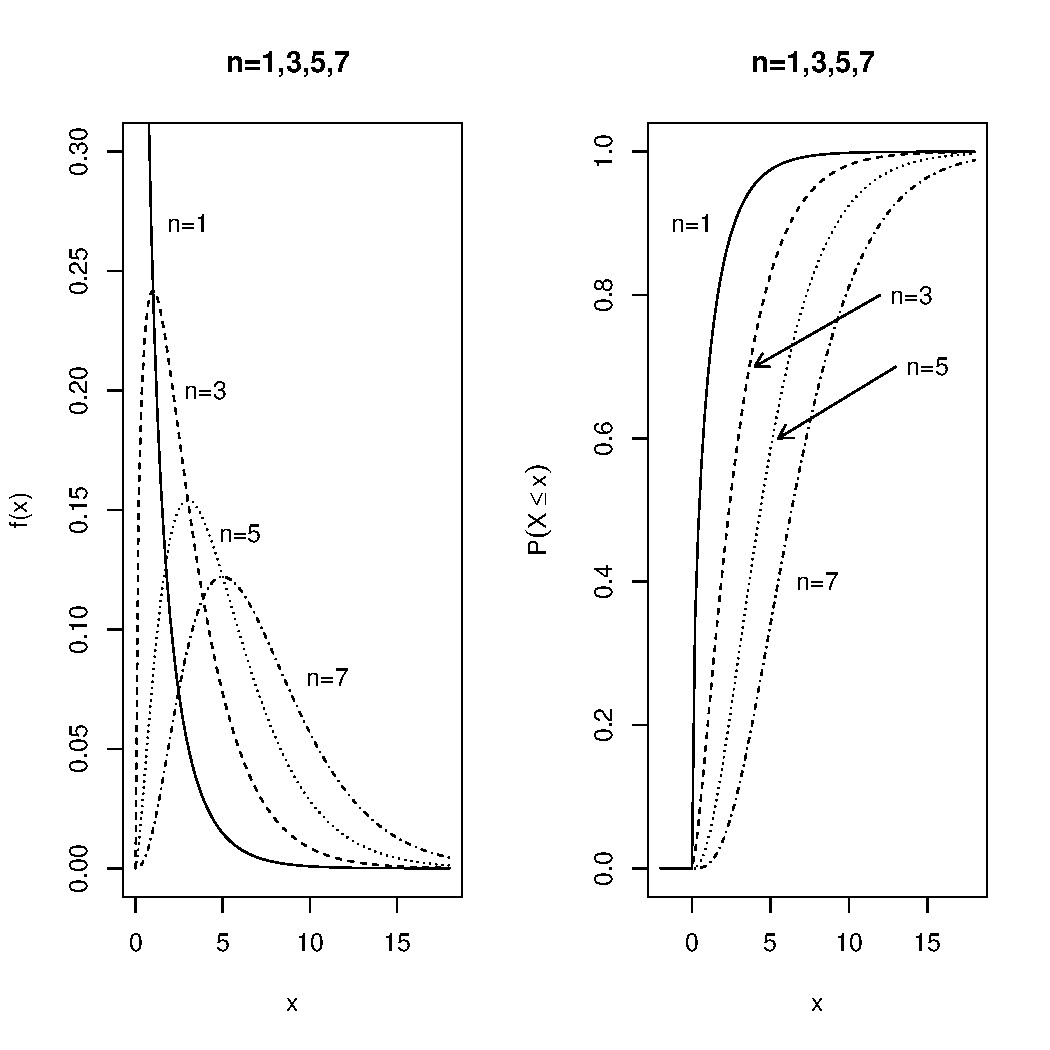
\includegraphics[height=16cm]{capitoli/images/4_chiquadrato/densProbChi.pdf}
    \caption{Densità di probabilità e funzione di distribuzione}
\end{figure}

In molti problemi reali, si desidera verificare se il campione osservato può essere stato estratto da una popolazione descritta da una variabile aleatoria $X$ con funzione di distribuzione $F_X(x)$. A questo scopo, si utilizza il criterio di verifica delle ipotesi del chi-quadrato, detto anche test del chi-quadrato o test del buon adattamento.

\section{Criterio del chi-quadrato bilaterale}

Con il criterio del  chi-quadrato si desidera verificare l'ipotesi che una certa popolazione, descritta da una variabile aleatoria $X$, sia caratterizzata da una funzione di distribuzione $F_X(x)$ con $k$ parametri non noti da stimare. Denotando con $H_0$ l'ipotesi soggetta a verifica (ipotesi nulla) e con $H_1$ l'ipotesi alternativa, il test chi-quadrato di misura $\alpha$ mira a verificare l'ipotesi nulla.

$H_0:X$ ha una funzione di distribuzione $F_X(x)$ (avendo stimato k parametri non noti in base al campione) 

in alternativa all'ipotesi

$H_1:X$ non ha una funzione di distribuzione $F_X(x)$ dove $\alpha$ è la probabilità massima di rifiutare l'ipotesi nulla quando essa è vera.

Anche in questo caso si determina un test $\phi$ di misura $\alpha$ che permetta di determinare una regione di accettazione e di rifiuto dell'ipotesi nulla. 

Si suddivida l'insieme dei valori che la variabile aleatoria $X$ può assumere in $r$ sottoinsiemi $I_1, I_2, ..., I_r$ in modo che risulti essere uguale a $p_i$ la probabilità che, secondo la distribuzione ipotizzata, la variabile aleatoria assuma un valore appartenente a $I_i$, ossia

\[p_i = P(X \in I_i) \quad (i=1,2,...,r\].

Lo step successivo, preso un campione $x_1, x_2, ..., x_n$ è di calcolare le frequenze assolute $n_2, ..., n_r$ con cui gli $n$ elementi si distribuiscono nei rispettivi insiemi $I_1, I_2, ..., I_r$. Il numero medio di elementi che cadono nell'intervallo $I_i$ è $np_i$. Si calcola poi la quantità

\[x^2 = \sum_{i=1}^r(\frac{n_i - np_i}{\sqrt{np_i}})^2\]

Il criterio chi-quadrato si basa sulla statistica

\[Q = \sum_{i=1}^r(\frac{N_i - np_i}{\sqrt{np_i}})^2\]

dove $N_i$ è la variabile aleatoria che descrive il numero degli elementi del campione casuale $X_1, X_2, ..., X_n$ (costituito da $n$ variabili  aleatorie osservabili, indipendenti e identicamente distribuite con la stessa legge di probabilità $F_X(x)$ della popolazione) che cadono nell'intervallo $I_i(i=1,2,...,r)$.

Se la variabile aleatoria $X$ ha una funzione di distribuzione $F_X(x)$ con $k$ parametri non noti, si può dimostrare che per $n$ sufficientemente grande la funzione di distribuzione della statistica $Q$ è approssimabile con la funzione di distribuzione chi-quadrato con $r-k-1$ gradi di libertà.

Per garantire che ogni classe contenga almeno 5 elementi, si ritiene valida l'approssimazione se risulta 

\[min(np_1, np_2, ..., np_r) \geq 5\]

Si giunge così alla definizione del test chi-quadrato bilaterale. Per un campione sufficientemente numeroso di ampiezza $n$, il test chi-quadrato bilaterale di misura $\alpha$ è il seguente:

\begin{itemize}
    \item si rifiuti l'ipotesi $H_0 se \chi^2 < \chi_{1-\alpha/2,r-k-1}^2$ oppure $\chi^2 > \chi_{\alpha/2, r-k-1}^2$;
    \item si accetti l'ipotesi $\chi_{1-\alpha/2,r-k-1}^2 < \chi^2 < \chi_{\alpha/2, r-k-1}^2$
\end{itemize}

dove $\chi_{1-\alpha/2,r-k-1}^2$ e $\chi_{\alpha/2,r-k-1}^2$ sono soluzioni dele equazioni:

\[P(Q<\chi_{1-\alpha/2,r-k-1}^2) = \frac{\alpha}{2}, \quad P(Q<\chi_{\alpha/2,r-k-1}^2) = 1-\frac{\alpha}{2}\]

\noindent \textbf{Esempio}

\begin{lstlisting}
[1] 2.5889415 2.4274552 2.2879886 2.5257274 1.3608815 1.8330865 2.2110392
[8] 2.9302882 2.1603784 2.8153400 1.2379034 1.3232095 1.5533711 1.1738130
[15] 1.1798547 2.0803117 1.4592185 1.5569350 1.4902865 2.0316545 2.4187870
[22] 2.5316882 3.0833015 1.8875859 1.5517724 3.0869650 2.1161441 2.2039643
[29] 1.0669755 2.0200946 2.5388058 2.3822110 2.1206882 1.6142661 2.3803540
[36] 2.4263595 2.8091048 1.5316683 1.6807372 2.7404029 1.5801006 1.8411243
[43] 1.9379254 2.2090764 1.8581314 2.2168108 2.4149075 1.8682822 2.4080365
[50] 2.5663934 1.7010245 1.8328371 1.9498204 1.5384879 1.6274098 2.4448616
[57] 1.6637135 3.1919928 1.2788193 1.6247899 1.8259281 2.1353790 2.0575756
[64] 2.2415920 2.6733718 1.0493558 1.7638138 2.3932882 1.8392844 2.2664697
[71] 1.8736283 1.3277308 1.8608656 2.1320640 1.3944918 1.5087226 2.2219716
[78] 0.9680605 2.1960015 1.8015670

  n <- length(ds)
  n
  [1] 80

  m <- mean(ds)
  m
  [1] 1.996316

  d <- sd(ds)
  d
  [1] 0.51082
\end{lstlisting}

Applicando il test chi-quadrato di misura $\alpha = 0.05$ si desidera verificare se la popolazione da cui proviene il campione può essere descritta da una variabile aleatoria $X$ di densità normale

\[f_X(x) = \frac{1}{\delta \sqrt{2\pi}}exp{-\frac{(x-\mu)^2}{2\delta^2}}, \quad x \in \mathbb{R} \quad (\mu \in \mathbb{R}, \delta>0)\]

Supponiamo di suddividere l'insieme dei valori che tale variabile aleatoria normale $X$ può assumere in $r=4$ sottoinsiemi $I_1, I_2, ..., I_4$ in modo che risulti essere uguale a $p_i=0.25$ la probabilità che $X$ assuma un valore appartenente a $I_i(i=1,2,...,4)$. La condizione è verificata essendo $npi = 80*0.25 = 20\geq4$. Ricordando che uno stimatore di $\mu$ è la media campionaria e uno stimatore di $\delta^2$ è la varianza campionaria, utilizzando i quantili della distribuzione normale possiamo determinare i sottoinsiemi $I_1, I_2, ..., I_4$

\begin{lstlisting}
  quantili <- numeric(3)
  for (i in 1:3)
    quantili[i] <- qnorm(0.25 * i, mean = m, sd = d)
  quantili

  [1] 1.651773 1.996316 2.340859
\end{lstlisting}

Gli intervalli $I_1, I_2,..., I_4$ sono:

\[I_1 = (-\inf, 1.65), \quad I_2=[1.65, 2.00)\]
\[I_3 = [2.00,2.34), \quad I_4 = [2.34,+\inf)\]

Occorre ora determinare il numero di elementi del campione che cadono negli intervalli $I_1, I_2, ..., I_4$:

\begin{lstlisting}
  r <- 4
  nint <- numeric(r)
  nint[1] <- length(which(ds < quantili[1]))
  nint[2] <- length(which((ds >= quantili[1]) & (ds < quantili[2])))
  nint[3] <- length(which((ds >= quantili[2]) & (ds < quantili[3])))
  nint[4] <- length(which((ds >= quantili[3])))
  nint

  [1] 23 17 18 22
\end{lstlisting}

Con il seguente codice si raffigurano le classi che suddividono il campione:

\begin{lstlisting}
  curve(dnorm(x, mean = m, sd = d), from = -1.25, to = 5.25,
        axes = FALSE, ylim = c(0, 0.8), xlab = "", ylab = "",
        main = "Densita normale mu = 1.99 sigma = 0.51")
  axis(side = 1, labels = FALSE)
  axis(side = 2, labels = TRUE)
  lines(x = quantili, y = dnorm(quantili, mean = m, sd = d), type = "h", lty = 2, xlab = "")
  axis(1, at = quantili, round(quantili, digits = 2), las = 2, cex.axis = 0.8)
\end{lstlisting}

\begin{figure}[!htbp]
    \centering
    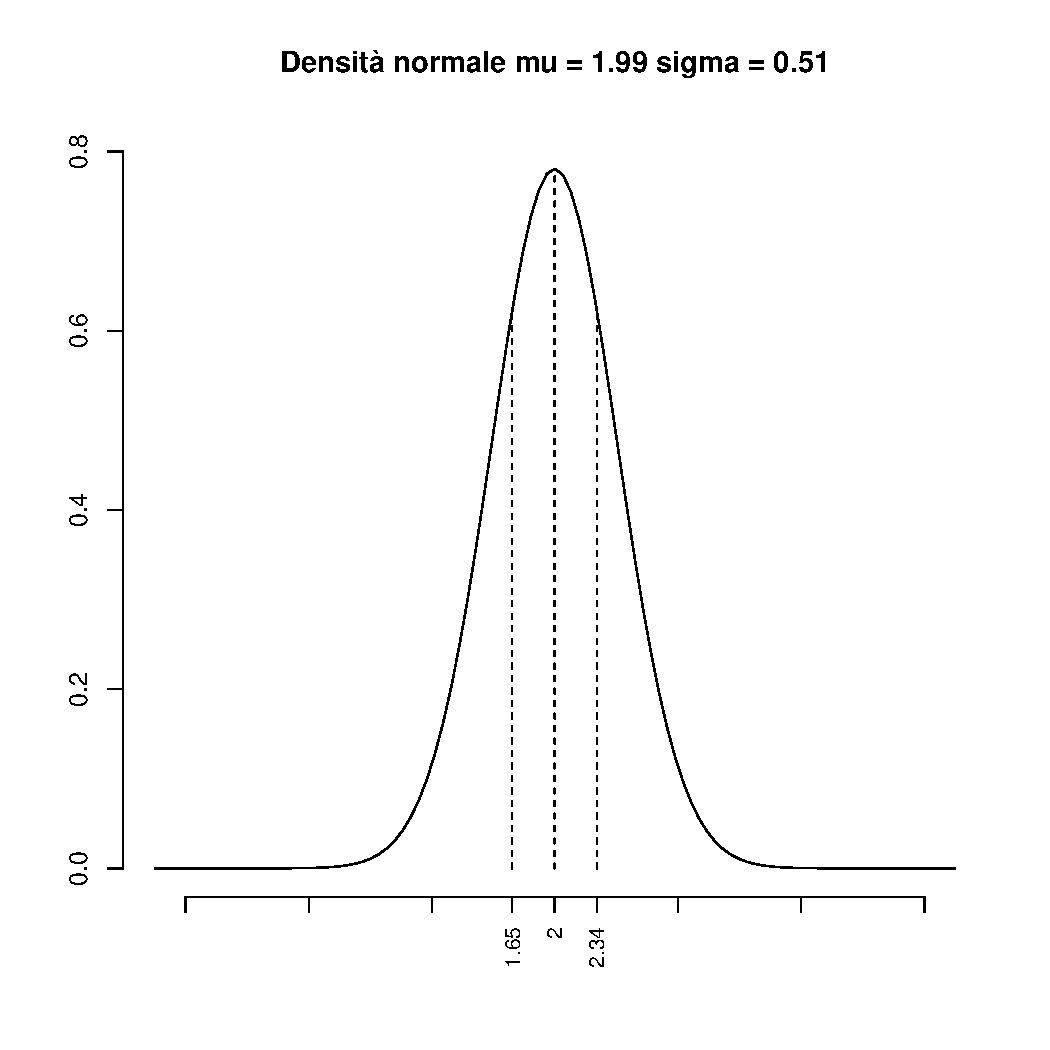
\includegraphics[height=16cm]{capitoli/images/4_chiquadrato/densNorm.pdf}
    \caption{Rappresentazione grafica dei 4 intervalli}
\end{figure}

Calcoliamo ora $\chi^2$

\begin{lstlisting}
  chi2 <- sum(((nint - n * 0.25) / sqrt(n * 0.25))^2)
  chi2
  [1] 1.3
\end{lstlisting}

La distribuzione normale ha due parametri non noti $(\mu, \delta^2)$ e quindi $k=2$. Pertanto, la funzione di distribuzione della statistica $Q$ è approssimabile con la funzione di distribuzione chi-quadrato con $r-k-1=2$ gradi di libertà. La funzione $qchisq$ permette di calcolare i quantili di una funzione di distribuzione chi-quadrato.

Occorre quindi calcolare $\chi_{\alpha/2,2}^2$ e $\chi_{1-\alpha/2,2}^2$ con $\alpha = 0.05$

\begin{lstlisting}
  k <- 2
  alpha <- 0.05
  qchisq(alpha / 2, df = r - k - 1)
  [1] 0.0009820691
  qchisq(1 - alpha / 2, df = r - k - 1)
  [1] 5.023886
\end{lstlisting}

da cui segue che $\chi_{\alpha/2,2}^2 = 0.000982$ e $\chi_{1-\alpha/2,2}^2 = 5.0239$. Essendo $0.000982 < 1.3 < 5.0239$ l'ipotesi $H_0$ di popolazione normale deve essere accettata. Di seguito la rappresentazione grafica della regione di accettazione.

\begin{lstlisting}
  curve(dchisq(x, df = 2), from = 0, to = 10, ylim = c(0, 0.6), xlab = "", axes = FALSE, ylab = "",
        main = "Densita di Chi-Quadrato con 2 gradi di liberta")
  axis(side = 1, labels = FALSE)
  axis(side = 2, labels = FALSE)
  axis(1, at = qchisq(alpha / 2, df = r - k - 1), "chi^2 alpha/2,2")
  axis(1, at = qchisq(1 - alpha / 2, df = r - k - 1), "chi^2 1-alpha/2,2")
  lines(x = c(0.0009820691, 5.023886), y = dchisq(c(0.0009820691, 5.023886), df = 2), type = "h", lty
    = 2, xlab = "")
  text(2, 0.04, expression("Reg. accettazione"))
  lines(x = 1.3, y = dchisq(1.3, df = 2), type = "h", lty = 2, xlab = "")
  axis(1, at = 1.3, "1.3")
\end{lstlisting}

\begin{figure}[!htbp]
    \centering
    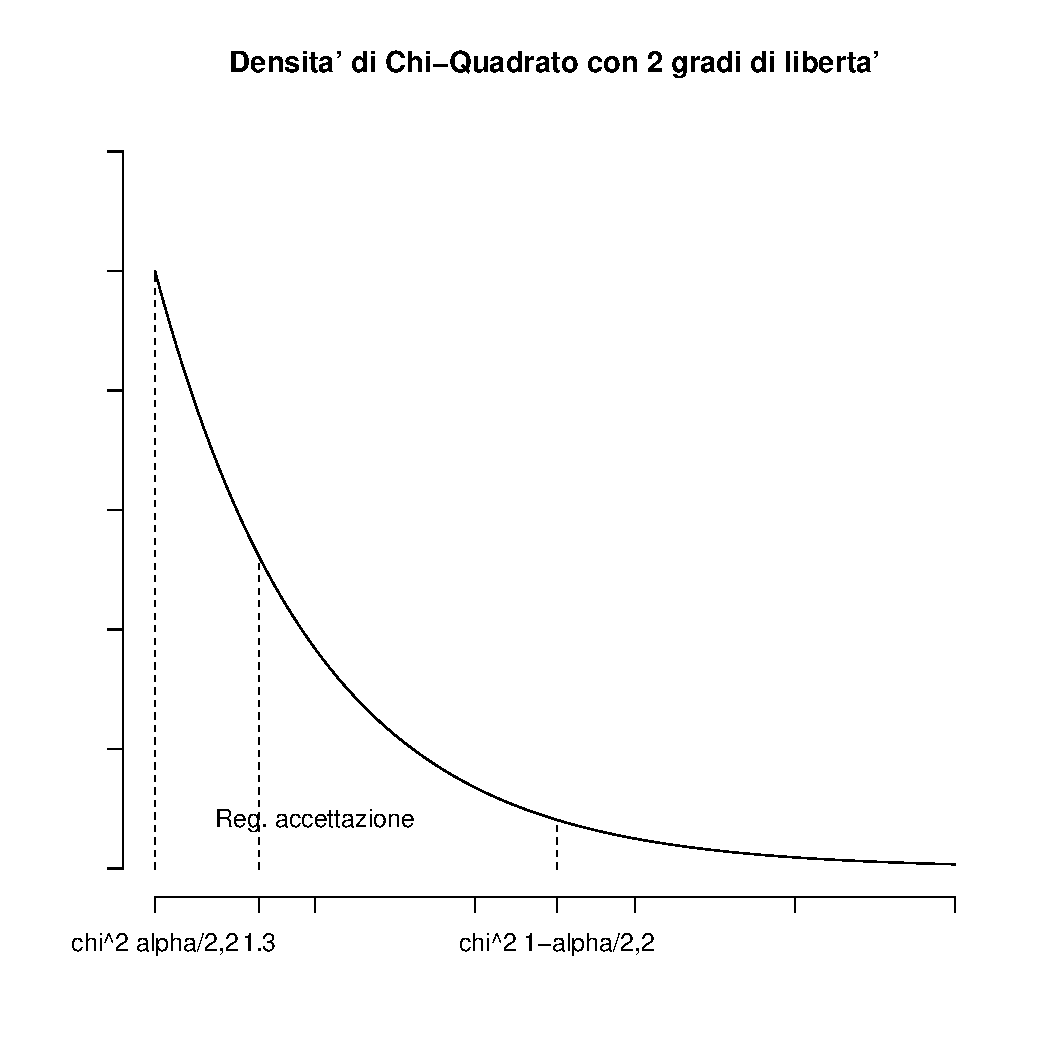
\includegraphics[height=16cm]{capitoli/images/4_chiquadrato/densChiFinal.pdf}
    \caption{ Regione di accettazione con grado di confidenza 0.05
}
\end{figure}

Essendo $0.000982 < \chi^2 < 5.0239$, l'ipotesi $H_0$ di popolazione normale può essere accettata.

%################################################

\newpage

\backmatter
\end{document}